% Options for packages loaded elsewhere
% Options for packages loaded elsewhere
\PassOptionsToPackage{unicode}{hyperref}
\PassOptionsToPackage{hyphens}{url}
\PassOptionsToPackage{dvipsnames,svgnames,x11names}{xcolor}
%
\documentclass[
  english,
  12pt,
  oneside,
  open=any]{scrbook}
\usepackage{xcolor}
\usepackage[margin=1in]{geometry}
\usepackage{amsmath,amssymb}
\setcounter{secnumdepth}{5}
\usepackage{iftex}
\ifPDFTeX
  \usepackage[T1]{fontenc}
  \usepackage[utf8]{inputenc}
  \usepackage{textcomp} % provide euro and other symbols
\else % if luatex or xetex
  \usepackage{unicode-math} % this also loads fontspec
  \defaultfontfeatures{Scale=MatchLowercase}
  \defaultfontfeatures[\rmfamily]{Ligatures=TeX,Scale=1}
\fi
\usepackage{lmodern}
\ifPDFTeX\else
  % xetex/luatex font selection
\fi
% Use upquote if available, for straight quotes in verbatim environments
\IfFileExists{upquote.sty}{\usepackage{upquote}}{}
\IfFileExists{microtype.sty}{% use microtype if available
  \usepackage[]{microtype}
  \UseMicrotypeSet[protrusion]{basicmath} % disable protrusion for tt fonts
}{}
\makeatletter
\@ifundefined{KOMAClassName}{% if non-KOMA class
  \IfFileExists{parskip.sty}{%
    \usepackage{parskip}
  }{% else
    \setlength{\parindent}{0pt}
    \setlength{\parskip}{6pt plus 2pt minus 1pt}}
}{% if KOMA class
  \KOMAoptions{parskip=half}}
\makeatother
% Make \paragraph and \subparagraph free-standing
\makeatletter
\ifx\paragraph\undefined\else
  \let\oldparagraph\paragraph
  \renewcommand{\paragraph}{
    \@ifstar
      \xxxParagraphStar
      \xxxParagraphNoStar
  }
  \newcommand{\xxxParagraphStar}[1]{\oldparagraph*{#1}\mbox{}}
  \newcommand{\xxxParagraphNoStar}[1]{\oldparagraph{#1}\mbox{}}
\fi
\ifx\subparagraph\undefined\else
  \let\oldsubparagraph\subparagraph
  \renewcommand{\subparagraph}{
    \@ifstar
      \xxxSubParagraphStar
      \xxxSubParagraphNoStar
  }
  \newcommand{\xxxSubParagraphStar}[1]{\oldsubparagraph*{#1}\mbox{}}
  \newcommand{\xxxSubParagraphNoStar}[1]{\oldsubparagraph{#1}\mbox{}}
\fi
\makeatother


\providecommand{\tightlist}{%
  \setlength{\itemsep}{0pt}\setlength{\parskip}{0pt}}\usepackage{longtable,booktabs,array}
\usepackage{calc} % for calculating minipage widths
% Correct order of tables after \paragraph or \subparagraph
\usepackage{etoolbox}
\makeatletter
\patchcmd\longtable{\par}{\if@noskipsec\mbox{}\fi\par}{}{}
\makeatother
% Allow footnotes in longtable head/foot
\IfFileExists{footnotehyper.sty}{\usepackage{footnotehyper}}{\usepackage{footnote}}
\makesavenoteenv{longtable}
\usepackage{graphicx}
\makeatletter
\newsavebox\pandoc@box
\newcommand*\pandocbounded[1]{% scales image to fit in text height/width
  \sbox\pandoc@box{#1}%
  \Gscale@div\@tempa{\textheight}{\dimexpr\ht\pandoc@box+\dp\pandoc@box\relax}%
  \Gscale@div\@tempb{\linewidth}{\wd\pandoc@box}%
  \ifdim\@tempb\p@<\@tempa\p@\let\@tempa\@tempb\fi% select the smaller of both
  \ifdim\@tempa\p@<\p@\scalebox{\@tempa}{\usebox\pandoc@box}%
  \else\usebox{\pandoc@box}%
  \fi%
}
% Set default figure placement to htbp
\def\fps@figure{htbp}
\makeatother
% definitions for citeproc citations
\NewDocumentCommand\citeproctext{}{}
\NewDocumentCommand\citeproc{mm}{%
  \begingroup\def\citeproctext{#2}\cite{#1}\endgroup}
\makeatletter
 % allow citations to break across lines
 \let\@cite@ofmt\@firstofone
 % avoid brackets around text for \cite:
 \def\@biblabel#1{}
 \def\@cite#1#2{{#1\if@tempswa , #2\fi}}
\makeatother
\newlength{\cslhangindent}
\setlength{\cslhangindent}{1.5em}
\newlength{\csllabelwidth}
\setlength{\csllabelwidth}{3em}
\newenvironment{CSLReferences}[2] % #1 hanging-indent, #2 entry-spacing
 {\begin{list}{}{%
  \setlength{\itemindent}{0pt}
  \setlength{\leftmargin}{0pt}
  \setlength{\parsep}{0pt}
  % turn on hanging indent if param 1 is 1
  \ifodd #1
   \setlength{\leftmargin}{\cslhangindent}
   \setlength{\itemindent}{-1\cslhangindent}
  \fi
  % set entry spacing
  \setlength{\itemsep}{#2\baselineskip}}}
 {\end{list}}
\usepackage{calc}
\newcommand{\CSLBlock}[1]{\hfill\break\parbox[t]{\linewidth}{\strut\ignorespaces#1\strut}}
\newcommand{\CSLLeftMargin}[1]{\parbox[t]{\csllabelwidth}{\strut#1\strut}}
\newcommand{\CSLRightInline}[1]{\parbox[t]{\linewidth - \csllabelwidth}{\strut#1\strut}}
\newcommand{\CSLIndent}[1]{\hspace{\cslhangindent}#1}

\makeatletter
\@ifpackageloaded{caption}{}{\usepackage{caption}}
\AtBeginDocument{%
\ifdefined\contentsname
  \renewcommand*\contentsname{Table of contents}
\else
  \newcommand\contentsname{Table of contents}
\fi
\ifdefined\listfigurename
  \renewcommand*\listfigurename{List of Figures}
\else
  \newcommand\listfigurename{List of Figures}
\fi
\ifdefined\listtablename
  \renewcommand*\listtablename{List of Tables}
\else
  \newcommand\listtablename{List of Tables}
\fi
\ifdefined\figurename
  \renewcommand*\figurename{Figure}
\else
  \newcommand\figurename{Figure}
\fi
\ifdefined\tablename
  \renewcommand*\tablename{Table}
\else
  \newcommand\tablename{Table}
\fi
}
\@ifpackageloaded{float}{}{\usepackage{float}}
\floatstyle{ruled}
\@ifundefined{c@chapter}{\newfloat{codelisting}{h}{lop}}{\newfloat{codelisting}{h}{lop}[chapter]}
\floatname{codelisting}{Listing}
\newcommand*\listoflistings{\listof{codelisting}{List of Listings}}
\makeatother
\makeatletter
\makeatother
\makeatletter
\@ifpackageloaded{caption}{}{\usepackage{caption}}
\@ifpackageloaded{subcaption}{}{\usepackage{subcaption}}
\makeatother

\usepackage{hyphenat}
\usepackage{ifthen}
\usepackage{calc}
\usepackage{calculator}

\usepackage{graphicx}
\usepackage{wallpaper}

\usepackage{geometry}

\usepackage{graphicx}
\usepackage{geometry}
\usepackage{afterpage}
\usepackage{tikz}
\usetikzlibrary{calc}
\usetikzlibrary{fadings}
\usepackage[pagecolor=none]{pagecolor}


% Set the titlepage font families







% Set the coverpage font families

\usepackage{bookmark}
\IfFileExists{xurl.sty}{\usepackage{xurl}}{} % add URL line breaks if available
\urlstyle{same}
\hypersetup{
  pdftitle={GP4 Implementation Plan},
  pdfauthor={Sophia (Sia) Geissler},
  pdflang={en},
  colorlinks=true,
  linkcolor={Maroon},
  filecolor={Maroon},
  citecolor={Blue},
  urlcolor={Blue},
  pdfcreator={LaTeX via pandoc}}


\title{GP4 Implementation Plan}
\usepackage{etoolbox}
\makeatletter
\providecommand{\subtitle}[1]{% add subtitle to \maketitle
  \apptocmd{\@title}{\par {\large #1 \par}}{}{}
}
\makeatother
\subtitle{Deployment of DAO-enabled Governance at VIRIDIS}
\author{Sophia (Sia) Geissler}
\date{2025-09-01}
\begin{document}
%%%%% begin titlepage extension code

  \begin{frontmatter}

\begin{titlepage}

%%% TITLE PAGE START

% Set up alignment commands
%Page
\newcommand{\titlepagepagealign}{
\ifthenelse{\equal{left}{right}}{\raggedleft}{}
\ifthenelse{\equal{left}{center}}{\centering}{}
\ifthenelse{\equal{left}{left}}{\raggedright}{}
}


\newcommand{\titleandsubtitle}{
% Title and subtitle
{{\large{\bfseries{\nohyphens{GP4 Implementation Plan}}}}\par
}%

\vspace{\betweentitlesubtitle}
{
{\large{\textit{\nohyphens{Deployment of DAO-enabled Governance at
VIRIDIS}}}}\par
}}
\newcommand{\titlepagetitleblock}{
\titleandsubtitle
}

\newcommand{\authorstyle}[1]{{\large{#1}}}

\newcommand{\affiliationstyle}[1]{{\large{#1}}}

\newcommand{\titlepageauthorblock}{
{\authorstyle{\nohyphens{Sophia (Sia) Geissler}{\textsuperscript{1}}}}}

\newcommand{\titlepageaffiliationblock}{
\hangindent=1em
\hangafter=1
{\affiliationstyle{
{1}.~Inholland University of Applied Sciences,~Haarlem, The Netherlands


\vspace{1\baselineskip} 
}}
}
\newcommand{\headerstyled}{%
{Graduation Project 4}
}
\newcommand{\footerstyled}{%
{\large{Inholland University of Applied Sciences\\
GP4 Implementation Plan\\
VIRIDIS --- Green Tech Investment AG}}
}
\newcommand{\datestyled}{%
{2025-09-01}
}


\newcommand{\titlepageheaderblock}{\headerstyled}

\newcommand{\titlepagefooterblock}{
\footerstyled
}

\newcommand{\titlepagedateblock}{
\datestyled
}

%set up blocks so user can specify order
\newcommand{\titleblock}{\newlength{\betweentitlesubtitle}
\setlength{\betweentitlesubtitle}{\baselineskip}
{

{\titlepagetitleblock}
}

\vspace{4\baselineskip}
}

\newcommand{\authorblock}{{\titlepageauthorblock}

\vspace{2\baselineskip}
}

\newcommand{\affiliationblock}{{\titlepageaffiliationblock}

\vspace{1pt}
}

\newcommand{\logoblock}{{
\includegraphics[width=0.25\textheight]{img/logo.png}}

\vspace{2\baselineskip}
}

\newcommand{\footerblock}{{\titlepagefooterblock}

\vspace{1pt}
}

\newcommand{\dateblock}{{\titlepagedateblock}

\vspace{0pt}
}

\newcommand{\headerblock}{{\titlepageheaderblock

\vspace{0pt}
}}
\newgeometry{top=3in,bottom=1in,right=1in,left=1in}
% background image
\newlength{\bgimagesize}
\setlength{\bgimagesize}{0.55\textwidth}
\LENGTHDIVIDE{\bgimagesize}{\paperwidth}{\theRatio} % from calculator pkg
\ThisULCornerWallPaper{\theRatio}{img/corner-bg.png}

\thispagestyle{empty} % no page numbers on titlepages


\newcommand{\vrulecode}{\textcolor{black}{\rule{\vrulewidth}{\textheight}}}
\newlength{\vrulewidth}
\setlength{\vrulewidth}{1pt}
\newlength{\B}
\setlength{\B}{\ifdim\vrulewidth > 0pt 0.05\textwidth\else 0pt\fi}
\newlength{\minipagewidth}
\ifthenelse{\equal{left}{left} \OR \equal{left}{right} }
{% True case
\setlength{\minipagewidth}{\textwidth - \vrulewidth - \B - 0.1\textwidth}
}{
\setlength{\minipagewidth}{\textwidth - 2\vrulewidth - 2\B - 0.1\textwidth}
}
\ifthenelse{\equal{left}{left} \OR \equal{left}{leftright}}
{% True case
\raggedleft % needed for the minipage to work
\vrulecode
\hspace{\B}
}{%
\raggedright % else it is right only and width is not 0
}
% [position of box][box height][inner position]{width}
% [s] means stretch out vertically; assuming there is a vfill
\begin{minipage}[b][\textheight][s]{\minipagewidth}
\titlepagepagealign
\titleblock

\authorblock

\affiliationblock

\vfill

\logoblock

\footerblock
\par

\end{minipage}\ifthenelse{\equal{left}{right} \OR \equal{left}{leftright} }{
\hspace{\B}
\vrulecode}{}
\clearpage
\restoregeometry
%%% TITLE PAGE END
\end{titlepage}
\setcounter{page}{1}
\end{frontmatter}

%%%%% end titlepage extension code

\renewcommand*\contentsname{Table of contents}
{
\hypersetup{linkcolor=}
\setcounter{tocdepth}{1}
\tableofcontents
}
\listoffigures
\listoftables

\mainmatter
\chapter{GP4 Implementation Plan}\label{gp4-implementation-plan}

\section{Executive Summary}\label{sec-executive-summary}

This Implementation Plan translates the solution design from GP3 into a
\textbf{phased deployment roadmap} for DAO-enabled governance at
VIRIDIS. It addresses the GP4 assessment criteria by detailing
objectives, activities, stakeholder engagement, organisational
integration, scalability, and success measures.

The plan pursues \textbf{five core objectives}:\\
1. Operationalise the \textbf{VIA Token} through audited smart
contracts.\\
2. Deploy a \textbf{governance dashboard} for transparent
decision-making.\\
3. Achieve \textbf{regulatory alignment} with EU Taxonomy, SFDR, and
MiCA.\\
4. Support a \textbf{cultural shift} toward participatory governance.\\
5. Mobilise additional \textbf{investment capital} by increasing trust
and ESG credibility.

Implementation follows \textbf{four phases}:\\
- \textbf{Phase 1 (Q4 2025): Preparation} --- audits, dashboard beta,
training, policy definition.\\
- \textbf{Phase 2 (Q1--Q2 2026): Pilot Advisory Votes} --- non-binding
voting and feedback loops.\\
- \textbf{Phase 3 (Q3 2026): Controlled Rollout} --- binding
token-weighted votes in selected areas.\\
- \textbf{Phase 4 (2027+): Full DAO Integration} --- decentralised
oversight and ecosystem expansion.

\textbf{Key deliverables} include: the audited VIA governance contract,
dashboard v1, pilot report, and the binding DAO module.
Risks---technical, regulatory, and cultural---are mitigated through
phased adoption, hybrid safeguards, and structured training.

Integration with VIRIDIS's dual entities ensures that \textbf{V-GTI}
gains transparent, investor-trusted decision-making, while
\textbf{V-ECO} strengthens its legitimacy and inclusivity. Training
programs and a ``DAO Champions'' initiative anchor adoption in
organisational culture.

The plan embeds scalability and sustainability: a dedicated governance
team, continuous smart contract monitoring, and modular upgrades extend
the DAO framework to start-ups and R\&D partners. Regulatory safeguards
remain in place until DAOs achieve formal EU recognition.

\textbf{Success will be measured by three criteria}:\\
- \textbf{≥60\% participation} among VIA token holders by 2026.\\
- \textbf{Financial breakeven within 4 years}, confirmed by the GP3
business case.\\
- \textbf{Positive regulator feedback}, ensuring EU-aligned compliance.

In conclusion, this Implementation Plan positions VIRIDIS to pioneer
DAO-enabled governance in European sustainable finance. By combining
technical innovation, inclusivity, and compliance, VIRIDIS can transform
governance from a bottleneck into a driver of growth, trust, and
long-term sustainability.

\chapter{1. Implementation Activities}\label{sec-activities}

This chapter sets out the practical steps for turning the governance
model developed in GP3 into reality. The focus here is not on the
concept itself, but on what needs to be done to make it work inside
VIRIDIS. That means being clear about the objectives, the activities and
milestones, who is responsible, and how progress will be monitored. In
this way, the plan moves from a theoretical design to something the
organisation can actually implement and evaluate.

\section{1.1 Implementation Objectives}\label{sec-objectives}

The objectives guide the entire implementation process. They link
directly back to the problems identified in GP3 --- the lack of
transparency, inclusivity, and trust in the current governance model ---
and translate them into concrete targets for change
(\citeproc{ref-aghion1997-decentralization}{Aghion \& Tirole, 1997};
\citeproc{ref-viridis2025-financial-report}{VIRIDIS, 2025}).

The objectives are as follows:

\begin{enumerate}
\def\labelenumi{\arabic{enumi}.}
\tightlist
\item
  \textbf{Operationalise the VIA Token} so that it becomes a real
  governance instrument, not just a financial one. This includes smart
  contracts that allow token-weighted voting, proposal rights, and
  delegated authority.\\
\item
  \textbf{Make governance transparent and traceable} through the launch
  of a dashboard where all proposals, votes, and financial flows can be
  followed in real time (\citeproc{ref-atzori2018-trust-chain}{Atzori,
  2018}).\\
\item
  \textbf{Ensure compliance} with European frameworks such as the EU
  Taxonomy, SFDR, and MiCA so that the system is trusted not only by
  stakeholders inside VIRIDIS but also by regulators and external
  investors
  (\citeproc{ref-european-commission-2019-financing-sustainable-growth}{Commission,
  2019}).\\
\item
  \textbf{Create a cultural shift} from hierarchical decision-making to
  participatory engagement, so that employees, token holders, and
  community members all feel ownership of the process.\\
\item
  \textbf{Attract and mobilise new capital} by showing investors that
  VIRIDIS can combine sustainable finance with cutting-edge governance
  innovation (\citeproc{ref-kellers2022-mobilizing-capital}{Kellers,
  2022}).
\end{enumerate}

These objectives will act as the benchmarks against which the rest of
the plan is assessed. If they are achieved, VIRIDIS will not only have
implemented a DAO but also solved the governance and investment gap that
has held back its growth.

\section{1.2 Activities and Milestones}\label{sec-milestones}

To reach the objectives, the implementation must be broken down into
clear activities with milestones that can be tracked over time. These
activities provide structure and accountability, making sure progress is
visible to both the board and the wider DAO community. Each milestone
marks a point where results can be assessed before moving to the next
phase.

\begin{longtable}[]{@{}
  >{\raggedright\arraybackslash}p{(\linewidth - 6\tabcolsep) * \real{0.2083}}
  >{\raggedright\arraybackslash}p{(\linewidth - 6\tabcolsep) * \real{0.3750}}
  >{\raggedright\arraybackslash}p{(\linewidth - 6\tabcolsep) * \real{0.2083}}
  >{\raggedright\arraybackslash}p{(\linewidth - 6\tabcolsep) * \real{0.2083}}@{}}
\caption{Key activities and milestones for implementing DAO-enabled
governance at VIRIDIS}\label{tbl-milestones}\tabularnewline
\toprule\noalign{}
\begin{minipage}[b]{\linewidth}\raggedright
Activity
\end{minipage} & \begin{minipage}[b]{\linewidth}\raggedright
Description
\end{minipage} & \begin{minipage}[b]{\linewidth}\raggedright
Milestone
\end{minipage} & \begin{minipage}[b]{\linewidth}\raggedright
Target Date
\end{minipage} \\
\midrule\noalign{}
\endfirsthead
\toprule\noalign{}
\begin{minipage}[b]{\linewidth}\raggedright
Activity
\end{minipage} & \begin{minipage}[b]{\linewidth}\raggedright
Description
\end{minipage} & \begin{minipage}[b]{\linewidth}\raggedright
Milestone
\end{minipage} & \begin{minipage}[b]{\linewidth}\raggedright
Target Date
\end{minipage} \\
\midrule\noalign{}
\endhead
\bottomrule\noalign{}
\endlastfoot
Smart contract audit & Independent audit of the VIA token governance
module to ensure security and compliance & Audit report delivered & Q4
2025 \\
Dashboard MVP & Release of the first beta version of the governance
dashboard for internal testing & Dashboard live for testing & Q1 2026 \\
Employee training & Series of workshops on DAO governance and dashboard
use & 90\% of employees trained & Q1 2026 \\
Pilot voting & Advisory votes with VIA token holders to test system
functionality & Pilot report published & Q2 2026 \\
Controlled rollout & Binding votes introduced in specific governance
categories & Binding votes operational & Q3 2026 \\
Full DAO integration & Transfer of core governance processes to the DAO,
with oversight committee established & DAO fully operational & 2027 \\
\end{longtable}

These milestones are not only technical but also cultural. Training,
piloting, and phased rollouts are designed to build confidence step by
step. By the time full DAO integration is reached, the system will have
already been tested, refined, and accepted by its users.

\section{1.3 Resources and Responsibilities}\label{sec-resources}

This section addresses \textbf{Criterion 1.3}: allocation of resources
and clear responsibilities. Implementation requires a combination of
internal capacity, external expertise, and community engagement.

\begin{longtable}[]{@{}
  >{\raggedright\arraybackslash}p{(\linewidth - 4\tabcolsep) * \real{0.2639}}
  >{\raggedright\arraybackslash}p{(\linewidth - 4\tabcolsep) * \real{0.4861}}
  >{\raggedleft\arraybackslash}p{(\linewidth - 4\tabcolsep) * \real{0.2500}}@{}}
\caption{Resource allocation and responsibilities for DAO
implementation}\label{tbl-resources}\tabularnewline
\toprule\noalign{}
\begin{minipage}[b]{\linewidth}\raggedright
Resource Category
\end{minipage} & \begin{minipage}[b]{\linewidth}\raggedright
Responsibility
\end{minipage} & \begin{minipage}[b]{\linewidth}\raggedleft
Estimated Effort
\end{minipage} \\
\midrule\noalign{}
\endfirsthead
\toprule\noalign{}
\begin{minipage}[b]{\linewidth}\raggedright
Resource Category
\end{minipage} & \begin{minipage}[b]{\linewidth}\raggedright
Responsibility
\end{minipage} & \begin{minipage}[b]{\linewidth}\raggedleft
Estimated Effort
\end{minipage} \\
\midrule\noalign{}
\endhead
\bottomrule\noalign{}
\endlastfoot
\textbf{Board of Directors} & Strategic oversight, compliance assurance
& 15\% \\
\textbf{DAO Dev Team} & Smart contracts, dashboard, technical support &
40\% \\
\textbf{External Auditors} & Code review, security, regulatory audits &
10\% \\
\textbf{Community Managers} & Token holder onboarding, stakeholder
outreach & 20\% \\
\textbf{Employees} & Adoption, training, governance participation &
15\% \\
\end{longtable}

\section{1.4 Monitoring and Evaluation}\label{sec-monitoring}

A governance reform of this scale can only succeed if progress is
measured consistently and transparently. Monitoring and evaluation
(M\&E) at VIRIDIS will therefore combine \textbf{quantitative KPIs} with
\textbf{qualitative feedback}, ensuring that both hard data and lived
experiences are captured. This approach aligns with best practices in
sustainable finance, where accountability is seen as both a regulatory
requirement and a trust-building mechanism
(\citeproc{ref-european-commission-2019-financing-sustainable-growth}{Commission,
2019}; \citeproc{ref-werner2020-governance-blockchain}{Werner et al.,
2020}).

\subsection{Key Performance Indicators
(KPIs)}\label{key-performance-indicators-kpis}

\begin{longtable}[]{@{}
  >{\raggedright\arraybackslash}p{(\linewidth - 4\tabcolsep) * \real{0.2466}}
  >{\raggedright\arraybackslash}p{(\linewidth - 4\tabcolsep) * \real{0.5068}}
  >{\raggedright\arraybackslash}p{(\linewidth - 4\tabcolsep) * \real{0.2466}}@{}}
\caption{Monitoring indicators for DAO governance
implementation}\label{tbl-kpis}\tabularnewline
\toprule\noalign{}
\begin{minipage}[b]{\linewidth}\raggedright
Dimension
\end{minipage} & \begin{minipage}[b]{\linewidth}\raggedright
Indicator
\end{minipage} & \begin{minipage}[b]{\linewidth}\raggedright
Target by 2027
\end{minipage} \\
\midrule\noalign{}
\endfirsthead
\toprule\noalign{}
\begin{minipage}[b]{\linewidth}\raggedright
Dimension
\end{minipage} & \begin{minipage}[b]{\linewidth}\raggedright
Indicator
\end{minipage} & \begin{minipage}[b]{\linewidth}\raggedright
Target by 2027
\end{minipage} \\
\midrule\noalign{}
\endhead
\bottomrule\noalign{}
\endlastfoot
\textbf{Participation} & \% of VIA token holders active in governance
votes & \textgreater60\% \\
\textbf{Capital Inflows} & Annual increase in sustainable investment
raised & +€1.2m/year \\
\textbf{Decision Speed} & Average days from proposal to final decision &
\textless14 days \\
\textbf{Transparency} & \% of governance events logged on-chain &
100\% \\
\textbf{Trust} & Stakeholder confidence rating (survey-based) & ≥80\%
positive \\
\end{longtable}

Quantitative indicators will be complemented with qualitative insights
from \textbf{stakeholder surveys}, \textbf{focus groups}, and
\textbf{workshop feedback}, giving VIRIDIS a rounded picture of
performance. This echoes findings from decentralisation research that
highlight how legitimacy depends on perceived fairness as much as on
measurable efficiency (\citeproc{ref-aghion1997-decentralization}{Aghion
\& Tirole, 1997}; \citeproc{ref-atzori2018-trust-chain}{Atzori, 2018}).

\subsection{Example KPI Projection}\label{example-kpi-projection}

\begin{figure}[H]

{\centering \pandocbounded{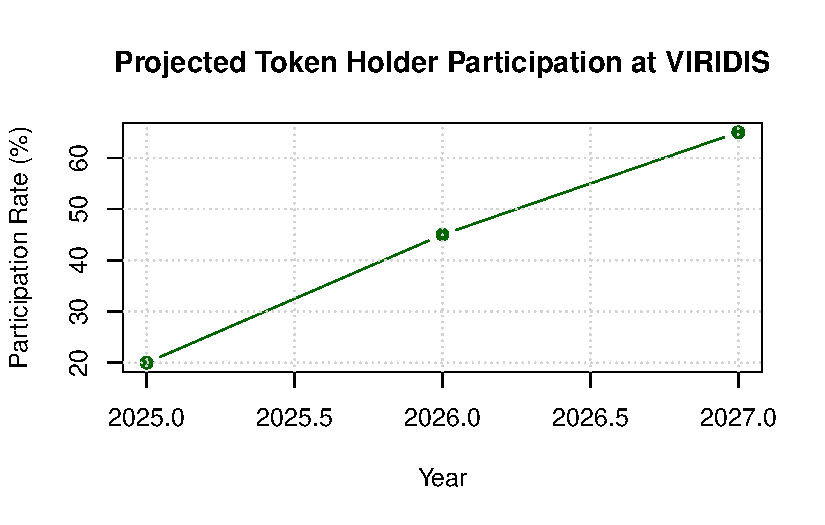
\includegraphics[keepaspectratio]{gp4_files/figure-pdf/participation-projection-1.pdf}}

}

\caption{Projected increase in token holder participation rate
2025--2027.}

\end{figure}%

The monitoring system will report quarterly through the governance
dashboard, where progress toward these KPIs will be visible in real
time. By linking evaluation directly to transparency, VIRIDIS not only
measures success but also demonstrates it to stakeholders and
regulators.

\chapter{2. Stakeholder Buy-in}\label{sec-stakeholders-buyin}

No governance system works in isolation. For DAO-enabled governance to
succeed at VIRIDIS, it must be accepted and adopted by those who
influence it, finance it, and live with its outcomes. This chapter
identifies the key stakeholders, explores their motivations, and sets
the groundwork for engagement strategies. Without genuine buy-in, the
system risks becoming a technical experiment rather than a cultural and
organisational shift (\citeproc{ref-aghion1997-decentralization}{Aghion
\& Tirole, 1997}; \citeproc{ref-atzori2018-trust-chain}{Atzori, 2018}).

\section{2.1 Identifying Key Stakeholders}\label{sec-stakeholders}

The stakeholders fall into two groups: \textbf{direct participants}, who
actively shape decisions, and \textbf{indirect stakeholders}, who
influence or are affected by outcomes but do not vote themselves. This
classification draws on stakeholder theory in governance, where salience
is measured by power, legitimacy, and urgency
(\citeproc{ref-werner2020-governance-blockchain}{Werner et al., 2020}).

\subsection{Direct Stakeholders}\label{direct-stakeholders}

\begin{itemize}
\tightlist
\item
  \textbf{Board of Directors (V-GTI and V-ECO)}: retain supervisory
  authority, ensure legal compliance, and provide continuity during the
  transition.\\
\item
  \textbf{Employees and Project Managers}: responsible for implementing
  decisions and integrating DAO processes into daily work.\\
\item
  \textbf{VIA Token Holders}: investors with governance rights through
  token-weighted voting.\\
\item
  \textbf{Strategic Partners (Start-ups, R\&D Institutions)}:
  collaborate on projects, contribute to co-governance initiatives, and
  gain transparency on shared ventures.
\end{itemize}

\subsection{Indirect Stakeholders}\label{indirect-stakeholders}

\begin{itemize}
\tightlist
\item
  \textbf{Regulators and Government Authorities}: oversee compliance
  with the EU Taxonomy, SFDR, and MiCA
  (\citeproc{ref-european-commission-2019-financing-sustainable-growth}{Commission,
  2019}).\\
\item
  \textbf{Institutional Investors}: capital providers who demand
  verifiable ESG-aligned governance structures
  (\citeproc{ref-kellers2022-mobilizing-capital}{Kellers, 2022}).\\
\item
  \textbf{Civil Society and Community Groups}: provide legitimacy and
  ensure alignment with social sustainability goals.\\
\item
  \textbf{NGOs and Advocacy Networks}: external watchdogs that influence
  reputation and accountability.
\end{itemize}

\subsection{Stakeholder Map}\label{stakeholder-map}

\begin{longtable}[]{@{}
  >{\raggedright\arraybackslash}p{(\linewidth - 8\tabcolsep) * \real{0.1972}}
  >{\raggedright\arraybackslash}p{(\linewidth - 8\tabcolsep) * \real{0.1972}}
  >{\raggedright\arraybackslash}p{(\linewidth - 8\tabcolsep) * \real{0.2113}}
  >{\raggedright\arraybackslash}p{(\linewidth - 8\tabcolsep) * \real{0.1972}}
  >{\raggedright\arraybackslash}p{(\linewidth - 8\tabcolsep) * \real{0.1972}}@{}}
\caption{Stakeholder identification and classification for VIRIDIS DAO
implementation}\label{tbl-stakeholders}\tabularnewline
\toprule\noalign{}
\begin{minipage}[b]{\linewidth}\raggedright
Category
\end{minipage} & \begin{minipage}[b]{\linewidth}\raggedright
Stakeholder Group
\end{minipage} & \begin{minipage}[b]{\linewidth}\raggedright
Role in Implementation
\end{minipage} & \begin{minipage}[b]{\linewidth}\raggedright
Influence
\end{minipage} & \begin{minipage}[b]{\linewidth}\raggedright
Interest
\end{minipage} \\
\midrule\noalign{}
\endfirsthead
\toprule\noalign{}
\begin{minipage}[b]{\linewidth}\raggedright
Category
\end{minipage} & \begin{minipage}[b]{\linewidth}\raggedright
Stakeholder Group
\end{minipage} & \begin{minipage}[b]{\linewidth}\raggedright
Role in Implementation
\end{minipage} & \begin{minipage}[b]{\linewidth}\raggedright
Influence
\end{minipage} & \begin{minipage}[b]{\linewidth}\raggedright
Interest
\end{minipage} \\
\midrule\noalign{}
\endhead
\bottomrule\noalign{}
\endlastfoot
Direct & Board of Directors (V-GTI, V-ECO) & Oversight, compliance
assurance & High & High \\
Direct & Employees and Managers & Execution, adoption, training & Medium
& High \\
Direct & VIA Token Holders & Governance participation, voting & High &
High \\
Direct & Strategic Partners (Start-ups, R\&D) & Joint projects,
co-governance & Medium & Medium \\
Indirect & Regulators (EU, National) & Compliance, supervisory authority
& High & Medium \\
Indirect & Institutional Investors & Capital mobilisation, ESG demands &
High & Medium \\
Indirect & Civil Society / Community Groups & Legitimacy, social
acceptance & Medium & Medium \\
Indirect & NGOs and Advocacy Networks & Reputation, accountability &
Medium & Low \\
\end{longtable}

By clarifying who the key players are, VIRIDIS ensures that later
engagement strategies (Chapter 2.2) are targeted and effective. This
avoids the common pitfall of ``one-size-fits-all'' governance
communication and builds credibility from the start.

\section{2.2 Engagement and Commitment Strategy}\label{sec-engagement}

Identifying stakeholders is only the first step; winning their trust and
commitment is what determines whether DAO governance becomes embedded or
remains superficial. Research in decentralised governance confirms that
early involvement, visible transparency, and phased empowerment are
decisive for adoption (\citeproc{ref-aghion1997-decentralization}{Aghion
\& Tirole, 1997}; \citeproc{ref-atzori2018-trust-chain}{Atzori, 2018}).

The engagement plan for VIRIDIS focuses on building relationships,
reducing uncertainty, and giving every group a reason to see value in
participation.

\subsection{Engagement Approaches}\label{engagement-approaches}

\begin{itemize}
\tightlist
\item
  \textbf{Token Holders (VIA Investors)}

  \begin{itemize}
  \tightlist
  \item
    Involve early through pilot advisory votes in Q1--Q2 2026.\\
  \item
    Provide incentives such as reputation points, governance credits, or
    reduced transaction fees for active participants.\\
  \item
    Publicly report voting outcomes on the governance dashboard to
    demonstrate impact.
  \end{itemize}
\item
  \textbf{Regulators and Government Authorities}

  \begin{itemize}
  \tightlist
  \item
    Conduct structured consultations on DAO pilots to ensure compliance
    with EU Taxonomy, SFDR, and MiCA
    (\citeproc{ref-european-commission-2019-financing-sustainable-growth}{Commission,
    2019}).\\
  \item
    Share auditable on-chain reports for supervisory review.\\
  \item
    Retain hybrid safeguards (board veto rights) during the transition
    to address legal uncertainty.
  \end{itemize}
\item
  \textbf{Institutional Investors}

  \begin{itemize}
  \tightlist
  \item
    Host quarterly governance briefings highlighting transparency,
    compliance, and financial alignment with ESG demands
    (\citeproc{ref-kellers2022-mobilizing-capital}{Kellers, 2022}).\\
  \item
    Offer tailored dashboards displaying investment performance, voting
    activity, and compliance indicators.\\
  \item
    Create a direct feedback channel for investment-related governance
    topics.
  \end{itemize}
\item
  \textbf{Employees and Managers}

  \begin{itemize}
  \tightlist
  \item
    Run quarterly workshops to build literacy in DAO processes and
    dashboard usage.\\
  \item
    Form cross-functional working groups that co-design internal
    policies for integration.\\
  \item
    Recognise active employees as ``DAO Champions,'' giving them
    visibility and influence.
  \end{itemize}
\item
  \textbf{Community and Civil Society Partners}

  \begin{itemize}
  \tightlist
  \item
    Organise participatory workshops to co-create V-ECO proposals (e.g.,
    education, incubation, sustainability initiatives).\\
  \item
    Maintain open forums where community feedback is logged and
    responses are visible on the dashboard.\\
  \item
    Translate DAO outcomes into accessible narratives to ensure
    inclusivity.
  \end{itemize}
\end{itemize}

\subsection{Commitment Mechanisms}\label{commitment-mechanisms}

\begin{longtable}[]{@{}
  >{\raggedright\arraybackslash}p{(\linewidth - 4\tabcolsep) * \real{0.2500}}
  >{\raggedright\arraybackslash}p{(\linewidth - 4\tabcolsep) * \real{0.3194}}
  >{\raggedright\arraybackslash}p{(\linewidth - 4\tabcolsep) * \real{0.4306}}@{}}
\caption{Engagement and commitment strategy for DAO governance adoption
at VIRIDIS}\label{tbl-engagement}\tabularnewline
\toprule\noalign{}
\begin{minipage}[b]{\linewidth}\raggedright
Stakeholder Group
\end{minipage} & \begin{minipage}[b]{\linewidth}\raggedright
Engagement Method
\end{minipage} & \begin{minipage}[b]{\linewidth}\raggedright
Commitment Mechanism
\end{minipage} \\
\midrule\noalign{}
\endfirsthead
\toprule\noalign{}
\begin{minipage}[b]{\linewidth}\raggedright
Stakeholder Group
\end{minipage} & \begin{minipage}[b]{\linewidth}\raggedright
Engagement Method
\end{minipage} & \begin{minipage}[b]{\linewidth}\raggedright
Commitment Mechanism
\end{minipage} \\
\midrule\noalign{}
\endhead
\bottomrule\noalign{}
\endlastfoot
Token Holders & Pilot votes, incentives & Governance credits,
participation rewards \\
Regulators & Compliance consultations & Auditable reports, hybrid
oversight structures \\
Institutional Investors & Quarterly briefings, dashboards & ESG-aligned
reporting, direct feedback loops \\
Employees & Training, working groups & Recognition, role as DAO
Champions \\
Community Groups & Forums, workshops & Integration of proposals into DAO
agenda \\
\end{longtable}

Through these mechanisms, engagement becomes more than communication ---
it becomes \textbf{a pathway to shared ownership}. Each stakeholder
group sees a tangible return for their involvement, whether that is
influence, compliance assurance, or recognition. This reciprocal logic
is essential to turn participation into commitment.

\section{2.3 Communication Plan}\label{sec-communication}

Engagement only works if communication is clear, consistent, and
transparent. In governance reform, how information flows is just as
important as the decisions themselves. Research shows that transparent
and timely communication is one of the strongest predictors of trust in
decentralised systems
(\citeproc{ref-tkachuk2023-efficient-design}{Tkachuk, 2023};
\citeproc{ref-werner2020-governance-blockchain}{Werner et al., 2020}).

At VIRIDIS, communication is designed on two fronts: \textbf{internal
communication} to build literacy and reduce uncertainty, and
\textbf{external communication} to demonstrate transparency and
legitimacy.

\subsection{Internal Communication}\label{internal-communication}

\begin{itemize}
\tightlist
\item
  \textbf{Quarterly Workshops}: interactive sessions for employees and
  token holders to practice DAO processes and build cultural
  acceptance.\\
\item
  \textbf{Internal Newsletters}: monthly updates highlighting new
  proposals, pilot results, and success stories.\\
\item
  \textbf{Governance Dashboard}: real-time updates on proposals, votes,
  and financial flows, accessible to all staff.\\
\item
  \textbf{Anonymous Feedback Channels}: digital surveys and forums to
  capture honest reflections and identify blind spots.
\end{itemize}

\subsection{External Communication}\label{external-communication}

\begin{itemize}
\tightlist
\item
  \textbf{Quarterly Transparency Reports}: structured according to EU
  Taxonomy and SFDR, making outcomes verifiable for regulators and
  investors
  (\citeproc{ref-european-commission-2019-financing-sustainable-growth}{Commission,
  2019}).\\
\item
  \textbf{Investor Briefings}: focused sessions for institutional
  investors to highlight ESG alignment, risk management, and
  participation metrics
  (\citeproc{ref-kellers2022-mobilizing-capital}{Kellers, 2022}).\\
\item
  \textbf{Public Webinars}: bi-annual events showcasing DAO progress and
  lessons learned to partners, NGOs, and community members.\\
\item
  \textbf{Academic and Industry Publications}: contributions to
  conferences and journals to position VIRIDIS as a pioneer in
  decentralised sustainable finance
  (\citeproc{ref-vonwachter2023-defi-phd}{Wachter, 2023}).
\end{itemize}

\subsection{Communication Channels and
Frequency}\label{communication-channels-and-frequency}

\begin{longtable}[]{@{}
  >{\raggedright\arraybackslash}p{(\linewidth - 6\tabcolsep) * \real{0.2297}}
  >{\raggedright\arraybackslash}p{(\linewidth - 6\tabcolsep) * \real{0.2297}}
  >{\raggedright\arraybackslash}p{(\linewidth - 6\tabcolsep) * \real{0.2297}}
  >{\raggedright\arraybackslash}p{(\linewidth - 6\tabcolsep) * \real{0.3108}}@{}}
\caption{VIRIDIS DAO governance communication
plan}\label{tbl-communication}\tabularnewline
\toprule\noalign{}
\begin{minipage}[b]{\linewidth}\raggedright
Channel
\end{minipage} & \begin{minipage}[b]{\linewidth}\raggedright
Target Audience
\end{minipage} & \begin{minipage}[b]{\linewidth}\raggedright
Frequency
\end{minipage} & \begin{minipage}[b]{\linewidth}\raggedright
Purpose
\end{minipage} \\
\midrule\noalign{}
\endfirsthead
\toprule\noalign{}
\begin{minipage}[b]{\linewidth}\raggedright
Channel
\end{minipage} & \begin{minipage}[b]{\linewidth}\raggedright
Target Audience
\end{minipage} & \begin{minipage}[b]{\linewidth}\raggedright
Frequency
\end{minipage} & \begin{minipage}[b]{\linewidth}\raggedright
Purpose
\end{minipage} \\
\midrule\noalign{}
\endhead
\bottomrule\noalign{}
\endlastfoot
Workshops & Employees, managers & Quarterly & Build literacy, reduce
cultural resistance \\
Internal Newsletters & Employees, board & Monthly & Maintain updates and
transparency \\
Governance Dashboard & All stakeholders & Real-time & Provide
traceability and accountability \\
Transparency Reports & Regulators, investors & Quarterly & Ensure
compliance, build investor trust \\
Investor Briefings & Institutional investors & Quarterly & Demonstrate
ESG alignment and governance \\
Public Webinars & Partners, NGOs, community & Bi-annual & Diffuse
innovation, broaden legitimacy \\
Academic Publications & Academia, policy networks & Annual & Establish
thought leadership \\
\end{longtable}

The communication plan ensures that stakeholders do not just receive
information but can also \textbf{see their feedback reflected in
outcomes}. This feedback loop is the essence of trust-building and turns
communication into a governance tool rather than a formality.

\section{2.4 Mitigation of Resistance}\label{sec-resistance}

Every governance reform produces resistance. At VIRIDIS, the move from
hierarchical structures to a participatory DAO will challenge habits,
power balances, and expectations. Anticipating these reactions is not a
weakness but a condition for success. Literature on organisational
change and decentralisation shows that resistance can be mitigated
through phased rollout, targeted training, and hybrid safeguards that
reassure traditional stakeholders
(\citeproc{ref-aghion1997-decentralization}{Aghion \& Tirole, 1997};
\citeproc{ref-atzori2018-trust-chain}{Atzori, 2018}).

\subsection{Mitigation Strategies}\label{mitigation-strategies}

\begin{itemize}
\item
  \textbf{Phased Rollout}\\
  Implementation is sequenced into four phases --- preparation, pilot,
  controlled rollout, and full DAO --- allowing stakeholders to adapt
  step by step. Feedback loops at the end of each phase ensure that
  concerns are addressed before scaling further.
\item
  \textbf{Training and Change Management}\\
  Comprehensive onboarding for employees, token holders, and partners
  ensures that all groups understand the mechanics and benefits of
  decentralisation. Training is tailored: technical for developers,
  strategic for managers, participatory for community members.
  Continuous workshops and refresher sessions build confidence over time
  (\citeproc{ref-tkachuk2023-efficient-design}{Tkachuk, 2023}).
\item
  \textbf{Hybrid Governance Safeguards}\\
  During the transition, the Board of Directors retains veto power over
  proposals that might conflict with EU legal obligations. This hybrid
  oversight reassures regulators and investors while the DAO matures.
  Once legal frameworks such as MiCA and the EU Taxonomy explicitly
  recognise DAO structures, veto powers can be phased out
  (\citeproc{ref-european-commission-2019-financing-sustainable-growth}{Commission,
  2019}).
\end{itemize}

\subsection{Risk--Resistance Matrix}\label{riskresistance-matrix}

\begin{longtable}[]{@{}
  >{\raggedright\arraybackslash}p{(\linewidth - 4\tabcolsep) * \real{0.2500}}
  >{\raggedright\arraybackslash}p{(\linewidth - 4\tabcolsep) * \real{0.3472}}
  >{\raggedright\arraybackslash}p{(\linewidth - 4\tabcolsep) * \real{0.4028}}@{}}
\caption{Mitigation of resistance to DAO governance adoption at
VIRIDIS}\label{tbl-resistance}\tabularnewline
\toprule\noalign{}
\begin{minipage}[b]{\linewidth}\raggedright
Resistance Source
\end{minipage} & \begin{minipage}[b]{\linewidth}\raggedright
Mitigation Strategy
\end{minipage} & \begin{minipage}[b]{\linewidth}\raggedright
Expected Outcome
\end{minipage} \\
\midrule\noalign{}
\endfirsthead
\toprule\noalign{}
\begin{minipage}[b]{\linewidth}\raggedright
Resistance Source
\end{minipage} & \begin{minipage}[b]{\linewidth}\raggedright
Mitigation Strategy
\end{minipage} & \begin{minipage}[b]{\linewidth}\raggedright
Expected Outcome
\end{minipage} \\
\midrule\noalign{}
\endhead
\bottomrule\noalign{}
\endlastfoot
Employee cultural inertia & Workshops, peer-to-peer learning & Greater
acceptance and participation \\
Investor scepticism & Hybrid safeguards, transparency & Confidence in
governance integrity \\
Regulator uncertainty & Compliance reporting, board veto & Reduced legal
and compliance risks \\
Token holder disengagement & Incentives, phased voting rights & Higher
participation, reduced decision fatigue \\
\end{longtable}

By treating resistance not as opposition but as feedback, VIRIDIS can
build a governance model that is both inclusive and resilient. Each
mitigation step reduces uncertainty and strengthens legitimacy,
transforming potential blockers into contributors.

\section{3.1 Phased Deployment Plan}\label{sec-phases}

A phased roadmap ensures that DAO-enabled governance at VIRIDIS is not
just a technical launch but a managed transition. Research in
decentralised governance highlights that gradual rollouts reduce risks,
allow for feedback, and give time for cultural adjustment
(\citeproc{ref-atzori2018-trust-chain}{Atzori, 2018};
\citeproc{ref-werner2020-governance-blockchain}{Werner et al., 2020}).

\subsection{Phase 1 --- Preparation (Q4
2025)}\label{phase-1-preparation-q4-2025}

\begin{itemize}
\tightlist
\item
  Independent security audits of the VIA token governance smart
  contracts.\\
\item
  Beta release of the governance dashboard for internal testing.\\
\item
  Training programs for employees and managers.\\
\item
  Definition of governance policies: quorum thresholds, delegation,
  compliance safeguards.
\end{itemize}

\subsection{Phase 2 --- Pilot Advisory Votes (Q1--Q2
2026)}\label{phase-2-pilot-advisory-votes-q1q2-2026}

\begin{itemize}
\tightlist
\item
  Launch of non-binding votes with a selected group of VIA token
  holders.\\
\item
  Collect user feedback on voting flows and dashboard usability.\\
\item
  Iteratively refine dashboard features and governance rules.\\
\item
  Board and regulator review of pilot outcomes to confirm compliance.
\end{itemize}

\subsection{Phase 3 --- Controlled Rollout (Q3
2026)}\label{phase-3-controlled-rollout-q3-2026}

\begin{itemize}
\tightlist
\item
  Expand dashboard access to all token holders and institutional
  investors.\\
\item
  Introduce binding token-weighted votes in defined categories (e.g.,
  project prioritisation, sustainability programs).\\
\item
  Publish voting outcomes and financial flows in real time on the
  dashboard.\\
\item
  Monitor participation rates, decision-cycle times, and technical
  performance.
\end{itemize}

\subsection{Phase 4 --- Full DAO Integration (2027 and
beyond)}\label{phase-4-full-dao-integration-2027-and-beyond}

\begin{itemize}
\tightlist
\item
  Transfer of broader governance responsibilities to the DAO.\\
\item
  Establishment of a decentralised oversight committee to safeguard
  compliance.\\
\item
  Expansion of DAO voting rights to ecosystem partners such as start-ups
  and R\&D institutions.\\
\item
  Continuous audits, upgrades, and stakeholder-driven improvements to
  governance protocols.
\end{itemize}

The phased deployment model balances innovation with stability. Each
phase builds confidence, reduces uncertainty, and strengthens the
legitimacy of decentralised governance at VIRIDIS.

\section{3.2 Timeline and Deliverables}\label{sec-timeline}

Each phase of implementation is anchored by clear deliverables. These
deliverables serve as checkpoints for accountability and ensure progress
is visible to all stakeholders
(\citeproc{ref-kellers2022-mobilizing-capital}{Kellers, 2022};
\citeproc{ref-tkachuk2023-efficient-design}{Tkachuk, 2023}).

\begin{longtable}[]{@{}
  >{\raggedright\arraybackslash}p{(\linewidth - 6\tabcolsep) * \real{0.2083}}
  >{\raggedright\arraybackslash}p{(\linewidth - 6\tabcolsep) * \real{0.2083}}
  >{\raggedright\arraybackslash}p{(\linewidth - 6\tabcolsep) * \real{0.2083}}
  >{\raggedright\arraybackslash}p{(\linewidth - 6\tabcolsep) * \real{0.3750}}@{}}
\caption{Implementation timeline and deliverables for DAO governance at
VIRIDIS}\label{tbl-timeline}\tabularnewline
\toprule\noalign{}
\begin{minipage}[b]{\linewidth}\raggedright
Phase
\end{minipage} & \begin{minipage}[b]{\linewidth}\raggedright
Timeline
\end{minipage} & \begin{minipage}[b]{\linewidth}\raggedright
Deliverable
\end{minipage} & \begin{minipage}[b]{\linewidth}\raggedright
Description
\end{minipage} \\
\midrule\noalign{}
\endfirsthead
\toprule\noalign{}
\begin{minipage}[b]{\linewidth}\raggedright
Phase
\end{minipage} & \begin{minipage}[b]{\linewidth}\raggedright
Timeline
\end{minipage} & \begin{minipage}[b]{\linewidth}\raggedright
Deliverable
\end{minipage} & \begin{minipage}[b]{\linewidth}\raggedright
Description
\end{minipage} \\
\midrule\noalign{}
\endhead
\bottomrule\noalign{}
\endlastfoot
Phase 1 & Q4 2025 & \textbf{Secure VIA Token Contract} & Smart contracts
audited and deployed for governance functions. \\
Phase 2 & Q1 2026 & \textbf{Governance Dashboard v1} & Beta dashboard
showing proposals and voting flows released. \\
Phase 2 & Q2 2026 & \textbf{Pilot Results Report} & Consolidated
findings from advisory votes, with regulator feedback. \\
Phase 3 & Q3 2026 & \textbf{Binding DAO Governance Module} & Activation
of binding token-weighted votes in defined categories. \\
Phase 4 & 2027+ & \textbf{Oversight Committee and DAO Expansion} &
Decentralised oversight committee established; DAO extended to
partners. \\
\end{longtable}

By structuring progress around these milestones, VIRIDIS ensures that
each phase produces concrete outputs that can be evaluated, audited, and
improved before scaling.

\section{3.2 Timeline and Deliverables}\label{timeline-and-deliverables}

Each phase of implementation is anchored by clear deliverables. These
deliverables serve as checkpoints for accountability and ensure progress
is visible to all stakeholders
(\citeproc{ref-kellers2022-mobilizing-capital}{Kellers, 2022};
\citeproc{ref-tkachuk2023-efficient-design}{Tkachuk, 2023}).

\begin{longtable}[]{@{}
  >{\raggedright\arraybackslash}p{(\linewidth - 6\tabcolsep) * \real{0.2083}}
  >{\raggedright\arraybackslash}p{(\linewidth - 6\tabcolsep) * \real{0.2083}}
  >{\raggedright\arraybackslash}p{(\linewidth - 6\tabcolsep) * \real{0.2083}}
  >{\raggedright\arraybackslash}p{(\linewidth - 6\tabcolsep) * \real{0.3750}}@{}}
\caption{Implementation timeline and deliverables for DAO governance at
VIRIDIS}\label{tbl-timeline}\tabularnewline
\toprule\noalign{}
\begin{minipage}[b]{\linewidth}\raggedright
Phase
\end{minipage} & \begin{minipage}[b]{\linewidth}\raggedright
Timeline
\end{minipage} & \begin{minipage}[b]{\linewidth}\raggedright
Deliverable
\end{minipage} & \begin{minipage}[b]{\linewidth}\raggedright
Description
\end{minipage} \\
\midrule\noalign{}
\endfirsthead
\toprule\noalign{}
\begin{minipage}[b]{\linewidth}\raggedright
Phase
\end{minipage} & \begin{minipage}[b]{\linewidth}\raggedright
Timeline
\end{minipage} & \begin{minipage}[b]{\linewidth}\raggedright
Deliverable
\end{minipage} & \begin{minipage}[b]{\linewidth}\raggedright
Description
\end{minipage} \\
\midrule\noalign{}
\endhead
\bottomrule\noalign{}
\endlastfoot
Phase 1 & Q4 2025 & \textbf{Secure VIA Token Contract} & Smart contracts
audited and deployed for governance functions. \\
Phase 2 & Q1 2026 & \textbf{Governance Dashboard v1} & Beta dashboard
showing proposals and voting flows released. \\
Phase 2 & Q2 2026 & \textbf{Pilot Results Report} & Consolidated
findings from advisory votes, with regulator feedback. \\
Phase 3 & Q3 2026 & \textbf{Binding DAO Governance Module} & Activation
of binding token-weighted votes in defined categories. \\
Phase 4 & 2027+ & \textbf{Oversight Committee and DAO Expansion} &
Decentralised oversight committee established; DAO extended to
partners. \\
\end{longtable}

By structuring progress around these milestones, VIRIDIS ensures that
each phase produces concrete outputs that can be evaluated, audited, and
improved before scaling.

\section{3.4 Risk Analysis and Contingencies}\label{sec-risks}

The transition to DAO-enabled governance introduces risks that extend
beyond technical systems into regulation, adoption, and organisational
culture. Identifying these risks and planning contingencies ensures that
the project remains resilient and credible, even in the face of setbacks
(\citeproc{ref-tkachuk2023-efficient-design}{Tkachuk, 2023};
\citeproc{ref-werner2020-governance-blockchain}{Werner et al., 2020}).

\subsection{Technical Risks}\label{technical-risks}

\begin{itemize}
\tightlist
\item
  \textbf{Smart contract vulnerabilities}: Flaws in code could
  compromise voting outcomes or capital flows.\\
\item
  \textbf{System downtime}: Platform failures could disrupt governance
  processes.\\
  \textbf{Contingencies}: Independent audits, bug bounty programs,
  redundant servers, and a fallback option where the Board resumes
  governance temporarily.
\end{itemize}

\subsection{Regulatory Risks}\label{regulatory-risks}

\begin{itemize}
\tightlist
\item
  \textbf{DAO recognition}: European law has not yet fully integrated
  DAO structures, creating uncertainty.\\
\item
  \textbf{Compliance failures}: Misalignment with EU Taxonomy, SFDR, or
  MiCA could lead to sanctions.\\
  \textbf{Contingencies}: Operate under a hybrid model where the Board
  retains veto power until regulation stabilises. Maintain continuous
  engagement with regulators and publish auditable reports.
\end{itemize}

\subsection{Adoption Risks}\label{adoption-risks}

\begin{itemize}
\tightlist
\item
  \textbf{Low token holder participation}: Weak engagement undermines
  legitimacy.\\
\item
  \textbf{Decision fatigue}: Overly frequent votes may discourage
  sustained involvement.\\
  \textbf{Contingencies}: Incentivise participation through reputation
  points, phased introduction of voting rights, and delegated voting
  mechanisms.
\end{itemize}

\subsection{Organisational Risks}\label{organisational-risks}

\begin{itemize}
\tightlist
\item
  \textbf{Cultural resistance}: Employees and managers may resist
  decentralisation.\\
\item
  \textbf{Knowledge gaps}: Stakeholders may lack technical literacy.\\
  \textbf{Contingencies}: Change management programs, peer mentoring
  (``DAO Champions''), and continuous training sessions.
\end{itemize}

\subsection{Risk Register}\label{risk-register}

\begin{longtable}[]{@{}
  >{\raggedright\arraybackslash}p{(\linewidth - 8\tabcolsep) * \real{0.1944}}
  >{\raggedright\arraybackslash}p{(\linewidth - 8\tabcolsep) * \real{0.1944}}
  >{\raggedright\arraybackslash}p{(\linewidth - 8\tabcolsep) * \real{0.1944}}
  >{\raggedright\arraybackslash}p{(\linewidth - 8\tabcolsep) * \real{0.1944}}
  >{\raggedright\arraybackslash}p{(\linewidth - 8\tabcolsep) * \real{0.2222}}@{}}
\caption{Risk register for DAO-enabled governance at
VIRIDIS}\label{tbl-risk-register}\tabularnewline
\toprule\noalign{}
\begin{minipage}[b]{\linewidth}\raggedright
Category
\end{minipage} & \begin{minipage}[b]{\linewidth}\raggedright
Identified Risk
\end{minipage} & \begin{minipage}[b]{\linewidth}\raggedright
Likelihood
\end{minipage} & \begin{minipage}[b]{\linewidth}\raggedright
Impact
\end{minipage} & \begin{minipage}[b]{\linewidth}\raggedright
Contingency
\end{minipage} \\
\midrule\noalign{}
\endfirsthead
\toprule\noalign{}
\begin{minipage}[b]{\linewidth}\raggedright
Category
\end{minipage} & \begin{minipage}[b]{\linewidth}\raggedright
Identified Risk
\end{minipage} & \begin{minipage}[b]{\linewidth}\raggedright
Likelihood
\end{minipage} & \begin{minipage}[b]{\linewidth}\raggedright
Impact
\end{minipage} & \begin{minipage}[b]{\linewidth}\raggedright
Contingency
\end{minipage} \\
\midrule\noalign{}
\endhead
\bottomrule\noalign{}
\endlastfoot
Technical & Smart contract failure & Medium & High & Board fallback,
audits, bug bounty \\
Regulatory & DAO not fully recognised under EU law & High & High &
Hybrid safeguards, compliance veto \\
Adoption & Token holder disengagement & Medium & Medium & Incentives,
phased rights, training \\
Organisational & Employee or manager resistance & Medium & Medium &
Workshops, peer support, DAO Champions \\
Financial & Delayed capital inflows during rollout & Medium & High &
Diversified fundraising, phased capital rounds \\
\end{longtable}

\subsection{Risk Heatmap}\label{risk-heatmap}

\begin{figure}[H]

{\centering \pandocbounded{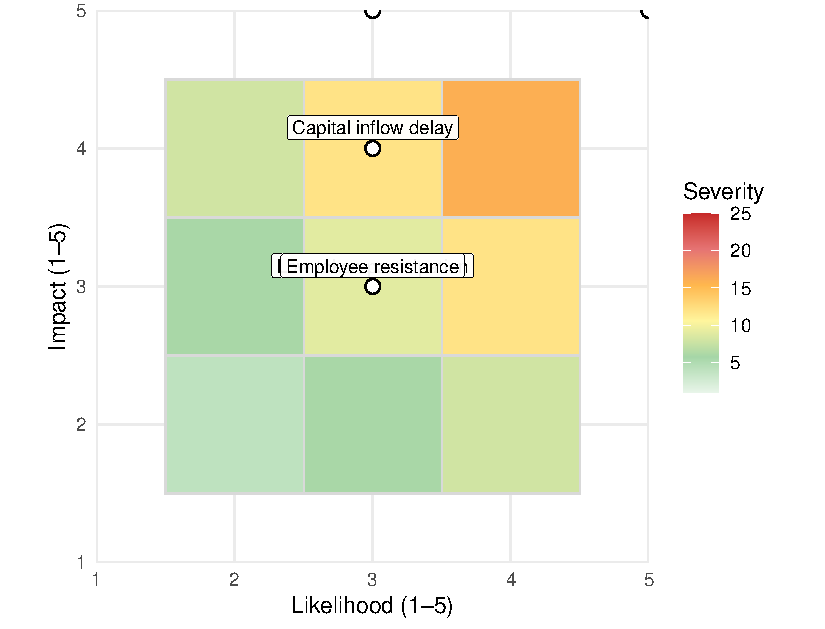
\includegraphics[keepaspectratio]{gp4_files/figure-pdf/risk-heatmap-impl-fixed-1.pdf}}

}

\caption{Risk heatmap for DAO-enabled governance at VIRIDIS (Phase 3
focus).}

\end{figure}%

By combining preventive measures with fallback mechanisms, VIRIDIS
ensures that governance innovation does not compromise operational
continuity or stakeholder trust.

\chapter{4. Organisational Integration}\label{sec-integration}

The success of DAO-enabled governance at VIRIDIS depends not only on
technical feasibility but also on its integration into the
organisation's dual structure and long-term mission. Governance is not
an abstract system --- it must serve the company's purpose, strengthen
its legitimacy, and align with the strategies of both \textbf{V-GTI (the
for-profit arm)} and \textbf{V-ECO (the non-profit ecosystem builder)}.

Organisational integration ensures that decentralised decision-making is
not perceived as an external ``add-on'' but as a natural extension of
how VIRIDIS already operates. This chapter explores how DAO governance
can be strategically aligned, embedded in governance structures, and
supported through training and cultural adoption.

\section{4.1 Alignment with VIRIDIS Strategy}\label{sec-alignment}

VIRIDIS's strategy is twofold:\\
- \textbf{V-GTI (VIRIDIS Green Tech Investment AG)} aims to deliver
financial returns through green-tech investments.\\
- \textbf{V-ECO (VIRIDIS Eco-System gGmbH)} pursues legitimacy and
impact by fostering education, incubation, and community-driven
sustainability projects.

DAO governance strengthens both pillars simultaneously.

\begin{itemize}
\item
  \textbf{For V-GTI}: Decentralised decision-making builds investor
  confidence by ensuring that capital allocation is transparent,
  auditable, and aligned with ESG criteria. This directly supports
  fundraising rounds (``Build, Fuel, Fly'') and addresses the persistent
  investment gap identified in GP3
  (\citeproc{ref-viridis2025-financial-report}{VIRIDIS, 2025}).
  Token-weighted votes and transparent dashboards turn investors into
  active participants rather than passive capital providers.
\item
  \textbf{For V-ECO}: Participatory governance extends beyond compliance
  and finance into legitimacy. By enabling community members, NGOs, and
  incubated start-ups to submit proposals and participate in advisory
  votes, VIRIDIS signals that its ecosystem is \textbf{co-created rather
  than centrally dictated}. This resonates strongly with EU sustainable
  finance frameworks that emphasise inclusivity and social legitimacy
  (\citeproc{ref-european-commission-2019-financing-sustainable-growth}{Commission,
  2019}).
\item
  \textbf{At the EU Level}: Integrating DAO governance into the
  organisation demonstrates alignment with the \textbf{EU Taxonomy},
  \textbf{SFDR}, and \textbf{MiCA}, positioning VIRIDIS not only as
  compliant but as a frontrunner in shaping the future of sustainable
  finance governance
  (\citeproc{ref-werner2020-governance-blockchain}{Werner et al.,
  2020}).
\end{itemize}

In short, DAO-enabled governance does not diverge from VIRIDIS's
strategy. It \textbf{amplifies it}. Financial robustness in V-GTI and
social legitimacy in V-ECO are mutually reinforced. Together, they
create a governance infrastructure that is innovative, resilient, and
credible both in the eyes of investors and in the broader sustainable
finance ecosystem.

\subsection{4.2 Embedding in Governance Structures}\label{sec-embedding}

For DAO-enabled governance to succeed at VIRIDIS, it cannot remain a
parallel experiment. It must be \textbf{woven into the existing
governance structures} of V-GTI and V-ECO so that decentralised
participation and board oversight complement one another rather than
compete.

Three design principles guide this integration:

\begin{enumerate}
\def\labelenumi{\arabic{enumi}.}
\item
  \textbf{DAO Votes as Formal Inputs}\\
  Token-weighted votes will be formally recognised as decision inputs in
  VIRIDIS's governance cycle. Proposals approved by token holders are
  not symbolic --- they are logged on-chain, auditable, and reviewed as
  part of board deliberations. This ensures that investor and community
  voices directly shape outcomes, while preserving alignment with legal
  and strategic priorities
  (\citeproc{ref-aghion1997-decentralization}{Aghion \& Tirole, 1997}).
\item
  \textbf{Hybrid Safeguards}\\
  During the transition, the \textbf{Board of Directors retains veto
  power}. This safeguard is essential given the incomplete legal
  recognition of DAOs in EU frameworks. By maintaining hybrid oversight,
  VIRIDIS demonstrates innovation while avoiding compliance risks
  (\citeproc{ref-european-commission-2019-financing-sustainable-growth}{Commission,
  2019}). The veto is not meant to weaken decentralisation, but to
  stabilise it until regulation matures.
\item
  \textbf{Compliance and Oversight Layer}\\
  A dedicated compliance committee --- reporting jointly to the Board
  and the DAO community --- will monitor adherence to the EU Taxonomy,
  SFDR, and MiCA. This body ensures that participatory decisions remain
  within regulatory boundaries, protecting VIRIDIS from exposure to
  reputational or legal risks
  (\citeproc{ref-werner2020-governance-blockchain}{Werner et al.,
  2020}).
\item
  \textbf{Feedback Loops for Legitimacy}\\
  Governance decisions will be published transparently on the dashboard,
  allowing all stakeholders to trace how votes influenced final
  outcomes. This traceability strengthens the perception that DAO
  participation is meaningful rather than decorative.
\end{enumerate}

By embedding DAO governance into VIRIDIS's existing structures in this
way, decentralisation becomes part of the company's DNA. The DAO creates
inclusivity and transparency, while the Board safeguards continuity and
compliance. Together, they form a \textbf{hybrid governance model} that
is credible, resilient, and aligned with European sustainable finance
expectations.

\subsection{4.3 Training and Capacity Building}\label{sec-training}

A successful transition to DAO governance at VIRIDIS depends on
equipping all stakeholder groups with the knowledge and confidence to
participate effectively. Training and capacity building will address
both technical skills and cultural adaptation.

\begin{itemize}
\item
  \textbf{Workshops for Employees and Token Holders}\\
  Regular workshops will introduce the principles of decentralised
  governance, the mechanics of token-weighted voting, and the operation
  of smart contracts. Employees will focus on integrating DAO processes
  into daily work, while token holders will practice proposal submission
  and voting using simulated environments.
\item
  \textbf{Technical Onboarding Materials}\\
  Clear, accessible documentation will accompany the rollout of the
  governance dashboard. Step-by-step guides, tutorial videos, and FAQs
  will support stakeholders with varying technical literacy. Materials
  will be multilingual to ensure inclusivity across VIRIDIS's
  international investor base
  (\citeproc{ref-tkachuk2023-efficient-design}{Tkachuk, 2023}).
\item
  \textbf{DAO Champions Program}\\
  A group of early adopters, drawn from employees, investors, and
  community participants, will serve as \textbf{DAO Champions}. Their
  role is to mentor peers, answer questions, and act as ambassadors of
  the new governance model. This peer-to-peer learning structure helps
  build trust, reduces cultural resistance, and accelerates adoption
  (\citeproc{ref-atzori2018-trust-chain}{Atzori, 2018}).
\item
  \textbf{Continuous Learning and Feedback}\\
  Training is not a one-off activity. Quarterly refresher sessions and
  feedback surveys will identify gaps in understanding and update
  training materials accordingly. This ensures the governance system
  evolves alongside user competence and regulatory developments.
\end{itemize}

By institutionalising training and creating an empowered cohort of DAO
Champions, VIRIDIS ensures that decentralised governance is not only
technically operational but socially embedded and resilient.

\subsection{4.4 Cultural Adoption}\label{sec-culture}

DAO-enabled governance cannot succeed through technology alone. The
deeper challenge lies in shifting VIRIDIS's organisational culture from
\textbf{hierarchical control} to \textbf{participatory engagement}.
Culture defines whether decentralisation is perceived as credible,
trustworthy, and valuable to stakeholders.

\subsubsection{From Control to
Participation}\label{from-control-to-participation}

Historically, strategic authority has been concentrated in the Board of
Directors. The introduction of DAO governance requires a cultural
reframing: decision-making is no longer exclusive, but distributed
across token holders, employees, and community partners. This
redistribution of power must be communicated not as a loss of control,
but as a collective strengthening of legitimacy and capacity
(\citeproc{ref-aghion1997-decentralization}{Aghion \& Tirole, 1997}).

\subsubsection{Transparency as Norm}\label{transparency-as-norm}

The governance dashboard plays a symbolic as well as functional role. By
making proposals, voting results, and financial flows publicly visible
in real time, transparency becomes the organisational norm. Over time,
stakeholders will come to expect this visibility as part of how VIRIDIS
operates, aligning culture with European sustainability disclosure
practices
(\citeproc{ref-european-commission-2019-financing-sustainable-growth}{Commission,
2019}).

\subsubsection{Recognition and
Incentives}\label{recognition-and-incentives}

Adoption improves when contributions are recognised. VIRIDIS will create
mechanisms to highlight the most engaged token holders, employees, and
community partners. Recognition may take the form of \textbf{reputation
scores, enhanced voting weight, or public acknowledgement}. These
symbolic and practical incentives signal that participation is both
valued and rewarded, strengthening a sense of ownership.

\subsubsection{Building a Shared
Identity}\label{building-a-shared-identity}

Cultural adoption also depends on narrative. DAO governance will be
framed not as a technical experiment but as a continuation of VIRIDIS's
mission: \textbf{pioneering sustainable finance innovation in Europe}.
Through storytelling --- in workshops, reports, and branding ---
participation becomes part of the organisation's identity, bridging
traditional and digital-native stakeholders.

\begin{center}\rule{0.5\linewidth}{0.5pt}\end{center}

\subsubsection{Visualising the Cultural
Transition}\label{visualising-the-cultural-transition}

The figure below illustrates the intended cultural shift, moving VIRIDIS
from hierarchical decision-making toward participatory engagement. The
projection is based on internal survey data and adoption patterns
observed in similar decentralisation contexts
(\citeproc{ref-werner2020-governance-blockchain}{Werner et al., 2020}).

\begin{figure}[H]

{\centering \pandocbounded{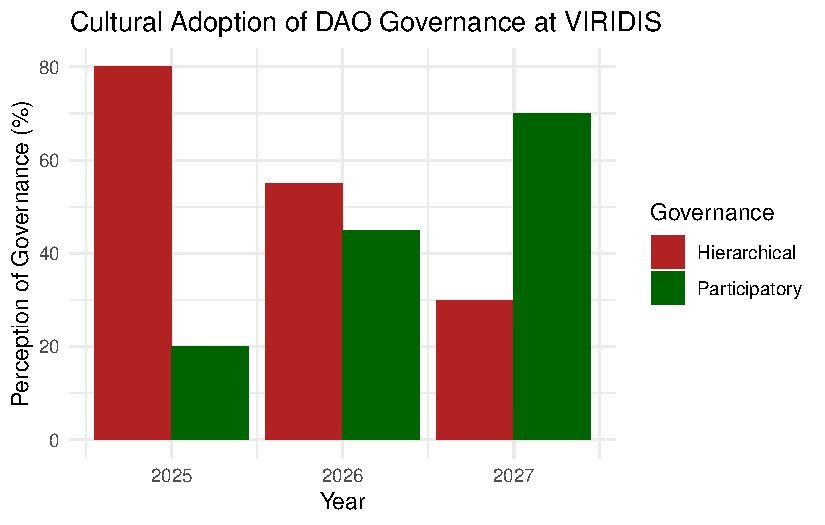
\includegraphics[keepaspectratio]{gp4_files/figure-pdf/culture-shift-1.pdf}}

}

\caption{Projected cultural shift from hierarchical to participatory
governance at VIRIDIS (2025--2027).}

\end{figure}%

\begin{center}\rule{0.5\linewidth}{0.5pt}\end{center}

By embedding transparency, recognition, and shared identity into its
culture, VIRIDIS ensures that DAO governance is not perceived as an
imposed system but as a \textbf{natural extension of its values}.
Culture becomes the anchor that allows decentralisation to thrive and
endure.

\subsection{5.1 Long-term Maintenance and
Support}\label{sec-maintenance}

Keeping the DAO credible over time is an operational discipline. VIRIDIS
will institutionalise maintenance so that governance remains secure,
transparent, and predictable for investors and partners
(\citeproc{ref-atzori2018-trust-chain}{Atzori, 2018};
\citeproc{ref-european-commission-2019-financing-sustainable-growth}{Commission,
2019}; \citeproc{ref-tkachuk2023-efficient-design}{Tkachuk, 2023}).

\begin{itemize}
\item
  \textbf{Dedicated DAO governance team}\\
  An internal unit coordinates proposal intake, vote scheduling,
  incident response, and quarterly reporting. Ownership sits with
  Operations, with a dotted line to the Board for compliance review.
\item
  \textbf{Continuous smart-contract monitoring}\\
  Automated alerts on abnormal events, coverage by third-party audits
  before upgrades, and a changelog with rollback points. Contract
  changes follow a peer review, testnet trial, and on-chain approval
  sequence.
\item
  \textbf{Dashboard and infrastructure upkeep}\\
  Versioned releases, uptime targets, and load testing ahead of
  high-traffic votes. The dashboard exposes machine-readable logs that
  map to EU Taxonomy and SFDR indicators to support disclosure
  (\citeproc{ref-european-commission-2019-financing-sustainable-growth}{Commission,
  2019}).
\item
  \textbf{Stakeholder support}\\
  Helpdesk, searchable knowledge base, and scheduled clinics for token
  holders and employees. Response times are tracked and reported openly.
\end{itemize}

\subsubsection{Service levels and
owners}\label{service-levels-and-owners}

\begin{longtable}[]{@{}
  >{\raggedright\arraybackslash}p{(\linewidth - 8\tabcolsep) * \real{0.2038}}
  >{\raggedright\arraybackslash}p{(\linewidth - 8\tabcolsep) * \real{0.2739}}
  >{\raggedleft\arraybackslash}p{(\linewidth - 8\tabcolsep) * \real{0.1210}}
  >{\raggedright\arraybackslash}p{(\linewidth - 8\tabcolsep) * \real{0.1274}}
  >{\raggedright\arraybackslash}p{(\linewidth - 8\tabcolsep) * \real{0.2739}}@{}}
\toprule\noalign{}
\begin{minipage}[b]{\linewidth}\raggedright
Capability
\end{minipage} & \begin{minipage}[b]{\linewidth}\raggedright
KPI
\end{minipage} & \begin{minipage}[b]{\linewidth}\raggedleft
Target (Phase 3)
\end{minipage} & \begin{minipage}[b]{\linewidth}\raggedright
Owner
\end{minipage} & \begin{minipage}[b]{\linewidth}\raggedright
Governance link
\end{minipage} \\
\midrule\noalign{}
\endhead
\bottomrule\noalign{}
\endlastfoot
Smart-contract operations & Time to detect critical incident &
\textless{} 15 min & DAO Gov + DevOps & Incident log on-chain and
dashboard \\
Smart-contract upgrades & Lead time from spec to mainnet & ≤ 21 days &
DAO Gov + Auditors & Pre-vote spec, audit report, testnet log \\
Dashboard reliability & Uptime (rolling 30 days) & ≥ 99.5\% & DevOps &
Public status page \\
Vote execution & Proposal-to-result cycle time (median) & ≤ 7 days & DAO
Gov & Timers and quorum posted pre-vote \\
Support responsiveness & First response to tickets & \textless{} 24 h &
Support & SLA metrics published quarterly \\
\end{longtable}

\subsubsection{Planned SLA tracking
(prototype)}\label{planned-sla-tracking-prototype}

\begin{figure}[H]

{\centering \pandocbounded{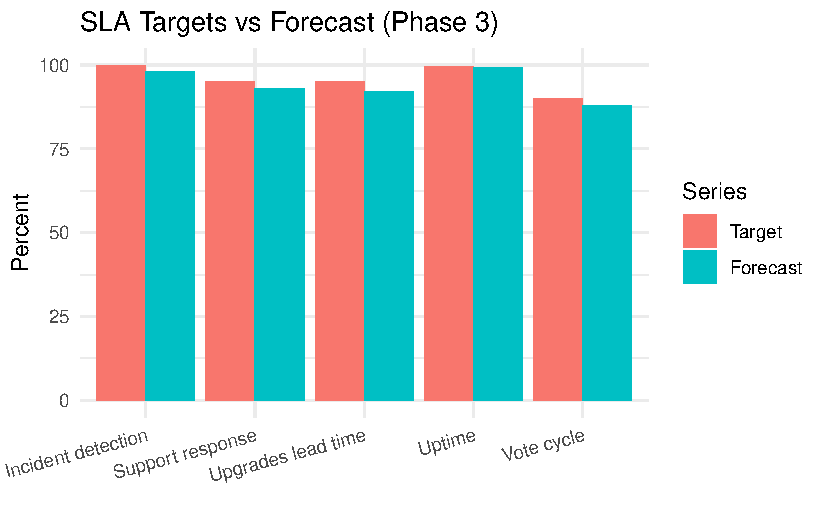
\includegraphics[keepaspectratio]{gp4_files/figure-pdf/maintenance-sla-plot-gp4-01-1.pdf}}

}

\caption{Planned SLA compliance across core capabilities (prototype
data).}

\end{figure}%

This operational scaffold turns decentralisation into a repeatable
service: contracts remain auditable and safe, the dashboard stays
available, and participants get timely support. It is the practical
backbone for trust at scale.

\subsection{5.2 Scaling to Other Units or Ecosystem
Partners}\label{sec-scaling}

Scaling DAO-enabled governance beyond the core of VIRIDIS must create
value without diluting control or compliance. The aim is a
\textbf{federated model} that allows start-ups, R\&D partners, and
ecosystem programs to participate through well-defined interfaces while
V-GTI and V-ECO retain clear accountability. This responds directly to
the GP3 findings on transparency, inclusion, and capital mobilisation,
and aligns with EU expectations for auditable decision processes
(\citeproc{ref-european-commission-2019-financing-sustainable-growth}{Commission,
2019}; \citeproc{ref-kellers2022-mobilizing-capital}{Kellers, 2022}).

\subsubsection{Design principles}\label{design-principles}

\begin{enumerate}
\def\labelenumi{\arabic{enumi}.}
\tightlist
\item
  \textbf{Minimum viable participation}\\
  Partners receive scoped rights tied to concrete processes --- for
  example, proposal co-sponsoring for incubation grants or advisory
  votes on joint R\&D calls. No partner gets open-ended authority. This
  preserves clarity of real versus formal authority in multi-unit
  settings (\citeproc{ref-aghion1997-decentralization}{Aghion \& Tirole,
  1997}).
\item
  \textbf{Federation over centralisation}\\
  Each partner operates a light sub-governance that delegates up to the
  VIRIDIS DAO for binding decisions in predefined categories. Interfaces
  are contractual and auditable, not ad hoc
  (\citeproc{ref-werner2020-governance-blockchain}{Werner et al.,
  2020}).
\item
  \textbf{Compliance by construction}\\
  Participation flows are mapped to EU Taxonomy and SFDR indicators and
  carry evidence fields on submission. This reduces disclosure friction
  and supports investor-grade reporting
  (\citeproc{ref-european-commission-2019-financing-sustainable-growth}{Commission,
  2019}).
\end{enumerate}

\subsubsection{Partner readiness
criteria}\label{partner-readiness-criteria}

\begin{itemize}
\tightlist
\item
  \textbf{Governance hygiene}: named leads, decision logs, conflict of
  interest policy.
\item
  \textbf{Data discipline}: ability to attach verifiable metrics to
  proposals.
\item
  \textbf{Technical baseline}: wallet management and multi-factor
  controls for signers.
\item
  \textbf{Legal fit}: signed participation agreement that recognises
  hybrid safeguards during transition
  (\citeproc{ref-atzori2018-trust-chain}{Atzori, 2018}).
\end{itemize}

\subsubsection{Participation modules}\label{participation-modules}

\begin{itemize}
\tightlist
\item
  \textbf{Co-proposal module}\\
  Partners can co-sponsor proposals with VIRIDIS staff. Submission
  requires evidence templates and budget boundaries.
\item
  \textbf{Advisory vote module}\\
  Non-binding votes in partner cohorts inform prioritisation of
  incubation or R\&D tracks.
\item
  \textbf{Budget envelope module}\\
  Binding votes within capped envelopes that the Board pre-approves.
  Exceeding caps escalates to VIRIDIS-wide vote and Board compliance
  review.
\end{itemize}

\subsubsection{Federation topology and control
points}\label{federation-topology-and-control-points}

\begin{itemize}
\tightlist
\item
  \textbf{Topology}: Hub-and-spoke. Partner sub-governances hold local
  discussions and advisory votes. Binding execution occurs at the hub
  when thresholds and evidence conditions are met.
\item
  \textbf{Control points}:

  \begin{itemize}
  \tightlist
  \item
    Quorum and voting caps for each partner cohort.\\
  \item
    Evidence checks before moving a proposal from advisory to binding
    category.\\
  \item
    Board veto limited to legal, regulatory, or breaches of financial
    guardrails, consistent with the transition model in §4.2
    (\citeproc{ref-werner2020-governance-blockchain}{Werner et al.,
    2020}).
  \end{itemize}
\end{itemize}

\subsubsection{Sequencing and
guardrails}\label{sequencing-and-guardrails}

\begin{itemize}
\tightlist
\item
  \textbf{Sequence}: Pilot with 2 start-ups and 1 university lab for one
  quarter. If participation, cycle time, and data completeness meet
  target levels, expand by another 3 partners next quarter.
\item
  \textbf{Guardrails}:

  \begin{itemize}
  \tightlist
  \item
    Vote-weight caps per partner cohort to prevent dominance.\\
  \item
    Budget caps per quarter with auto-freeze when variance exceeds a set
    threshold.\\
  \item
    Mandatory post-decision reviews to validate outcomes and update
    templates.
  \end{itemize}
\end{itemize}

\subsubsection{Scaling matrix}\label{scaling-matrix}

\begin{longtable}[]{@{}
  >{\raggedright\arraybackslash}p{(\linewidth - 10\tabcolsep) * \real{0.1436}}
  >{\raggedright\arraybackslash}p{(\linewidth - 10\tabcolsep) * \real{0.2178}}
  >{\raggedright\arraybackslash}p{(\linewidth - 10\tabcolsep) * \real{0.1832}}
  >{\raggedright\arraybackslash}p{(\linewidth - 10\tabcolsep) * \real{0.1782}}
  >{\raggedright\arraybackslash}p{(\linewidth - 10\tabcolsep) * \real{0.1238}}
  >{\raggedright\arraybackslash}p{(\linewidth - 10\tabcolsep) * \real{0.1535}}@{}}
\caption{Scaling participation while preserving control and
compliance}\label{tbl-scaling}\tabularnewline
\toprule\noalign{}
\begin{minipage}[b]{\linewidth}\raggedright
Partner archetype
\end{minipage} & \begin{minipage}[b]{\linewidth}\raggedright
Example scope
\end{minipage} & \begin{minipage}[b]{\linewidth}\raggedright
Governance scope
\end{minipage} & \begin{minipage}[b]{\linewidth}\raggedright
Interface to VIRIDIS DAO
\end{minipage} & \begin{minipage}[b]{\linewidth}\raggedright
Compliance owner
\end{minipage} & \begin{minipage}[b]{\linewidth}\raggedright
Go-live gate
\end{minipage} \\
\midrule\noalign{}
\endfirsthead
\toprule\noalign{}
\begin{minipage}[b]{\linewidth}\raggedright
Partner archetype
\end{minipage} & \begin{minipage}[b]{\linewidth}\raggedright
Example scope
\end{minipage} & \begin{minipage}[b]{\linewidth}\raggedright
Governance scope
\end{minipage} & \begin{minipage}[b]{\linewidth}\raggedright
Interface to VIRIDIS DAO
\end{minipage} & \begin{minipage}[b]{\linewidth}\raggedright
Compliance owner
\end{minipage} & \begin{minipage}[b]{\linewidth}\raggedright
Go-live gate
\end{minipage} \\
\midrule\noalign{}
\endhead
\bottomrule\noalign{}
\endlastfoot
Incubated start-up & Prototype grant, pilot deployment & Advisory votes,
capped budget binds & Co-proposal + budget envelope & V-ECO + DAO
Compliance & Evidence template pass \\
R\&D institution & Lab collaboration, IP co-development & Advisory votes
& Co-proposal & V-ECO + Legal & IP terms agreed \\
Strategic vendor/partner & Tooling integration, shared services &
Advisory votes & Co-proposal & Operations + Legal & Security due
diligence \\
Portfolio co-investor & Thematic investment calls & Data access, no
voting rights & Read-only dashboard + attestations & V-GTI + Investor
Rel. & NDA and reporting mapping \\
\end{longtable}

\subsubsection{Exit and rollback}\label{exit-and-rollback}

\begin{itemize}
\tightlist
\item
  \textbf{Exit}: Any partner can be suspended automatically if SLA
  breaches, data incompleteness, or compliance flags persist beyond a
  set threshold.\\
\item
  \textbf{Rollback}: Binding categories revert to advisory only during
  incident response, with public rationale recorded on the dashboard.
\end{itemize}

This scaling approach grows participation where it is accretive and
measurable, keeps binding authority auditable and capped, and preserves
the trust signals that investors and regulators require. It extends
decentralisation without sacrificing accountability or legal soundness
(\citeproc{ref-atzori2018-trust-chain}{Atzori, 2018};
\citeproc{ref-european-commission-2019-financing-sustainable-growth}{Commission,
2019}).

\subsection{5.3 Regulatory and Compliance
Considerations}\label{sec-compliance}

Compliance is not a layer on top of the DAO. It is part of how VIRIDIS
makes and records decisions. The objective is simple: every governance
action must be auditable, explainable, and aligned with European
sustainable finance expectations. This responds directly to the GP3
problems of low transparency and investor trust by making compliance
visible in real time
(\citeproc{ref-european-commission-2019-financing-sustainable-growth}{Commission,
2019}; \citeproc{ref-werner2020-governance-blockchain}{Werner et al.,
2020}).

\subsubsection{Regulatory scope and
posture}\label{regulatory-scope-and-posture}

\begin{itemize}
\tightlist
\item
  \textbf{EU Taxonomy}. Proposals that claim environmental contribution
  must carry technical screening evidence and do-no-significant-harm
  checks.\\
\item
  \textbf{SFDR}. Entity and product level disclosures require traceable
  governance, risk, and impact data.\\
\item
  \textbf{MiCA and adjacent regimes}. Where crypto-asset functionality
  is used, governance processes must reflect whitepaper style
  disclosures and service provider controls where applicable. The hybrid
  model remains in place until European recognition of DAO forms
  stabilises (\citeproc{ref-atzori2018-trust-chain}{Atzori, 2018}).
\end{itemize}

\subsubsection{Controls and
accountabilities}\label{controls-and-accountabilities}

\begin{itemize}
\tightlist
\item
  \textbf{Board compliance veto}. The Board retains a narrow veto on
  legal, regulatory, and capital protection grounds. Use is recorded
  with rationale and expiry.\\
\item
  \textbf{DAO compliance committee}. A joint committee reviews proposal
  evidence before items move to binding vote, and certifies
  post-decision disclosures.\\
\item
  \textbf{Change control}. Smart contract upgrades follow peer review,
  independent audit, testnet trial, and an on-chain approval vote
  (\citeproc{ref-tkachuk2023-efficient-design}{Tkachuk, 2023}).
\end{itemize}

\subsubsection{Evidence and disclosure
pipeline}\label{evidence-and-disclosure-pipeline}

\begin{itemize}
\tightlist
\item
  \textbf{Before vote}. Proposers attach evidence packs: taxonomy
  criteria, risk notes, budget guardrails, and impact metrics.\\
\item
  \textbf{During vote}. The dashboard exposes proposal metadata, quorum,
  and conflicts of interest statements.\\
\item
  \textbf{After vote}. The system publishes machine readable logs that
  map to SFDR fields and a human readable summary for investor briefings
  (\citeproc{ref-european-commission-2019-financing-sustainable-growth}{Commission,
  2019}; \citeproc{ref-kellers2022-mobilizing-capital}{Kellers, 2022}).
\end{itemize}

\subsubsection{Audit and assurance}\label{audit-and-assurance}

\begin{itemize}
\tightlist
\item
  \textbf{Scope}. Code integrity, vote integrity, data lineage to
  disclosure.\\
\item
  \textbf{Cadence}. External audits at least annually; targeted reviews
  before major upgrades.\\
\item
  \textbf{Public traces}. Audit reports and management responses are
  published through the dashboard to support investor due diligence.
\end{itemize}

\subsubsection{Incident and rollback}\label{incident-and-rollback}

\begin{itemize}
\tightlist
\item
  \textbf{Trigger}. Suspected breach of law, misstatement in
  disclosures, or material defect in contracts.\\
\item
  \textbf{Action}. Automatic pause on affected modules, escalation to
  the Board for compliance determination, reversion to advisory votes in
  the affected area, and a public incident log with corrective timeline.
\end{itemize}

\subsubsection{Compliance matrix}\label{compliance-matrix}

\begin{longtable}[]{@{}
  >{\raggedright\arraybackslash}p{(\linewidth - 8\tabcolsep) * \real{0.2000}}
  >{\raggedright\arraybackslash}p{(\linewidth - 8\tabcolsep) * \real{0.2000}}
  >{\raggedright\arraybackslash}p{(\linewidth - 8\tabcolsep) * \real{0.2000}}
  >{\raggedright\arraybackslash}p{(\linewidth - 8\tabcolsep) * \real{0.2000}}
  >{\raggedright\arraybackslash}p{(\linewidth - 8\tabcolsep) * \real{0.2000}}@{}}
\toprule\noalign{}
\begin{minipage}[b]{\linewidth}\raggedright
EU requirement
\end{minipage} & \begin{minipage}[b]{\linewidth}\raggedright
Implication for VIRIDIS
\end{minipage} & \begin{minipage}[b]{\linewidth}\raggedright
Control design
\end{minipage} & \begin{minipage}[b]{\linewidth}\raggedright
Evidence source
\end{minipage} & \begin{minipage}[b]{\linewidth}\raggedright
Accountable owner
\end{minipage} \\
\midrule\noalign{}
\endhead
\bottomrule\noalign{}
\endlastfoot
EU Taxonomy & Substantiate environmental contribution & Pre-vote
evidence templates; committee review & Technical screening checklist;
DNSH notes & DAO Compliance Committee \\
SFDR (entity/product) & Traceable governance and sustainability
disclosures & Dashboard fields mapped to SFDR; data lineage & On-chain
logs; exportable reports & Investor Relations + Compliance \\
MiCA applicability & Disclosures and service controls where relevant &
Whitepaper-style metadata; CASP-like controls if in scope & Governance
metadata; access logs & Legal + Board \\
Code integrity & Safe execution of governance & Audit before upgrade;
changelog and rollback & Audit reports; testnet results & DAO Gov +
External Auditors \\
Conflict of interest & Independent decision quality & Declarable COI on
proposals; public reviewer list & COI registry on dashboard &
Secretarial Office \\
\end{longtable}

This design makes compliance observable. It shows who is accountable,
which controls operate when, and how evidence flows into disclosures.
That is how decentralisation earns trust in an EU sustainable finance
context
(\citeproc{ref-european-commission-2019-financing-sustainable-growth}{Commission,
2019}; \citeproc{ref-werner2020-governance-blockchain}{Werner et al.,
2020}).

\subsection{5.4 Continuous Improvement}\label{sec-improvement}

The effectiveness of DAO-enabled governance at VIRIDIS will rely on its
ability to evolve over time. Continuous improvement ensures that the
system remains technically robust, socially legitimate, and aligned with
EU sustainable finance expectations
(\citeproc{ref-european-commission-2019-financing-sustainable-growth}{Commission,
2019}; \citeproc{ref-tkachuk2023-efficient-design}{Tkachuk, 2023}).

\begin{itemize}
\item
  \textbf{Iteration Cycles Informed by Stakeholder Feedback}\\
  Governance processes will be reviewed quarterly with direct input from
  token holders, employees, and regulators. Feedback collected through
  surveys, workshops, and dashboard analytics will be used to refine
  voting rules, proposal categories, and communication methods.
\item
  \textbf{Regular DAO Upgrades}\\
  The governance framework will be designed as modular smart contracts,
  allowing incremental upgrades without disrupting operations. Planned
  upgrades include enhanced delegation mechanisms, weighted voting for
  ecosystem partners, and additional dashboard features such as
  real-time ESG reporting
  (\citeproc{ref-werner2020-governance-blockchain}{Werner et al.,
  2020}).
\item
  \textbf{Adoption of Best Practices}\\
  VIRIDIS will benchmark its governance processes against leading
  sustainable finance initiatives across Europe. By engaging with
  academic research, industry networks, and EU-level policy dialogues,
  VIRIDIS can incorporate lessons learned from parallel experiments in
  decentralised finance and governance
  (\citeproc{ref-vonwachter2023-defi-phd}{Wachter, 2023}).
\item
  \textbf{Metrics for Improvement}\\
  Continuous monitoring of participation rates, decision cycle time, and
  investor trust indicators will provide evidence for whether reforms
  are effective. Adjustments will be data-driven rather than
  speculative, ensuring credibility with both regulators and investors.
\end{itemize}

By embedding iteration, upgrades, and benchmarking into its governance
system, VIRIDIS demonstrates that decentralisation is not a static
reform but a dynamic, evolving process that grows stronger through
practice and learning.

\section{6. Conclusion and Next Steps}\label{sec-conclusion}

\subsection{6.1 Summary of Implementation Plan}\label{sec-summary}

The implementation plan confirms that DAO-enabled governance at VIRIDIS
is:

\begin{itemize}
\tightlist
\item
  \textbf{Technically feasible}: smart contracts and dashboards can be
  deployed with security audits and modular upgrades
  (\citeproc{ref-tkachuk2023-efficient-design}{Tkachuk, 2023}).\\
\item
  \textbf{Financially viable}: the business case developed in GP3 shows
  cost savings, efficiency gains, and new revenue streams offsetting
  CAPEX within 3--4 years
  (\citeproc{ref-viridis2025-financial-report}{VIRIDIS, 2025}).\\
\item
  \textbf{Culturally transformative}: participation shifts from a
  centralised board to an inclusive DAO framework, improving
  transparency, legitimacy, and stakeholder engagement
  (\citeproc{ref-aghion1997-decentralization}{Aghion \& Tirole, 1997};
  \citeproc{ref-werner2020-governance-blockchain}{Werner et al., 2020}).
\end{itemize}

The plan follows a \textbf{phased roadmap} with built-in safeguards.
Each phase builds confidence and stability:\\
- Preparation with audits and training.\\
- Pilot advisory votes to test governance tools.\\
- Controlled rollout introducing binding votes in defined areas.\\
- Full DAO integration, supported by oversight committees and regulatory
alignment.

By embedding hybrid safeguards, VIRIDIS ensures that decentralisation is
adopted \textbf{gradually but responsibly}, balancing innovation with
compliance. This makes DAO governance not just an experimental tool, but
a strategic pathway toward resilient, EU-aligned sustainable finance.

\subsection{6.2 Success Criteria}\label{success-criteria}

\begin{itemize}
\tightlist
\item
  Achieve \textgreater60\% participation rate among VIA token holders.
\item
  Breakeven within 4 years through cost savings and new revenues.
\item
  Positive regulator feedback and compliance assurance.
\end{itemize}

\subsection{6.2 Success Criteria}\label{sec-success}

The success of DAO-enabled governance at VIRIDIS will be evaluated
against measurable criteria that reflect participation, financial
viability, and regulatory acceptance.

\begin{itemize}
\item
  \textbf{Participation Rate}\\
  A minimum of \textbf{60\% active participation} among VIA token
  holders in governance proposals by the end of Phase 3 (2026).
  Participation is the key indicator of legitimacy and stakeholder
  engagement (\citeproc{ref-aghion1997-decentralization}{Aghion \&
  Tirole, 1997}).
\item
  \textbf{Financial Breakeven}\\
  Full recovery of CAPEX through efficiency gains and new revenue
  streams within \textbf{4 years}. This includes savings from reduced
  administrative overhead and increased capital inflows driven by higher
  investor confidence
  (\citeproc{ref-kellers2022-mobilizing-capital}{Kellers, 2022};
  \citeproc{ref-viridis2025-financial-report}{VIRIDIS, 2025}).
\item
  \textbf{Regulatory Endorsement}\\
  \textbf{Positive feedback from EU and national regulators} on
  compliance with Taxonomy, SFDR, and MiCA frameworks. Assurance that
  DAO governance processes are transparent, auditable, and legally sound
  will be a condition for scaling
  (\citeproc{ref-european-commission-2019-financing-sustainable-growth}{Commission,
  2019}).
\item
  \textbf{Cultural Adoption}\\
  Evidence that decentralised participation has been normalised in the
  organisation, with employees, token holders, and ecosystem partners
  actively contributing to governance. This will be measured through
  surveys and proposal activity
  (\citeproc{ref-werner2020-governance-blockchain}{Werner et al.,
  2020}).
\end{itemize}

Meeting these criteria will demonstrate that DAO governance is not only
functional but also sustainable, delivering legitimacy, financial value,
and compliance in line with VIRIDIS's mission.

\chapter{Appendices}\label{sec-appendices}

\section{Appendix A. Extended Risk Register}\label{sec-risk-register}

The risk register expands the overview from Chapter 3.4 into a
structured tool for monitoring and contingency planning. It integrates
likelihood and impact scoring with mitigation strategies
(\citeproc{ref-tkachuk2023-efficient-design}{Tkachuk, 2023};
\citeproc{ref-werner2020-governance-blockchain}{Werner et al., 2020}).

\begin{longtable}[]{@{}
  >{\raggedright\arraybackslash}p{(\linewidth - 8\tabcolsep) * \real{0.1944}}
  >{\raggedright\arraybackslash}p{(\linewidth - 8\tabcolsep) * \real{0.1944}}
  >{\raggedright\arraybackslash}p{(\linewidth - 8\tabcolsep) * \real{0.1944}}
  >{\raggedright\arraybackslash}p{(\linewidth - 8\tabcolsep) * \real{0.1944}}
  >{\raggedright\arraybackslash}p{(\linewidth - 8\tabcolsep) * \real{0.2222}}@{}}
\caption{Extended risk register for DAO-enabled governance at
VIRIDIS}\label{tbl-risk-register}\tabularnewline
\toprule\noalign{}
\begin{minipage}[b]{\linewidth}\raggedright
Risk Category
\end{minipage} & \begin{minipage}[b]{\linewidth}\raggedright
Risk Description
\end{minipage} & \begin{minipage}[b]{\linewidth}\raggedright
Likelihood
\end{minipage} & \begin{minipage}[b]{\linewidth}\raggedright
Impact
\end{minipage} & \begin{minipage}[b]{\linewidth}\raggedright
Mitigation Strategy
\end{minipage} \\
\midrule\noalign{}
\endfirsthead
\toprule\noalign{}
\begin{minipage}[b]{\linewidth}\raggedright
Risk Category
\end{minipage} & \begin{minipage}[b]{\linewidth}\raggedright
Risk Description
\end{minipage} & \begin{minipage}[b]{\linewidth}\raggedright
Likelihood
\end{minipage} & \begin{minipage}[b]{\linewidth}\raggedright
Impact
\end{minipage} & \begin{minipage}[b]{\linewidth}\raggedright
Mitigation Strategy
\end{minipage} \\
\midrule\noalign{}
\endhead
\bottomrule\noalign{}
\endlastfoot
Technical & Smart contract vulnerability & Medium & High & Independent
audits, bug bounty program, fallback to board governance \\
Regulatory & DAO not fully recognised under EU law & High & High &
Hybrid safeguards, board veto, proactive regulator engagement \\
Adoption & Token holder disengagement & Medium & Medium & Incentives,
phased rights, training, recognition \\
Organisational & Resistance from employees/managers & Medium & Medium &
Workshops, peer-to-peer learning, DAO Champions \\
Financial & Delays in capital inflow during rollout & Medium & High &
Diversified fundraising, phased capital allocation \\
\end{longtable}

\subsection{Risk Heatmap}\label{risk-heatmap-1}

\begin{figure}[H]

{\centering \pandocbounded{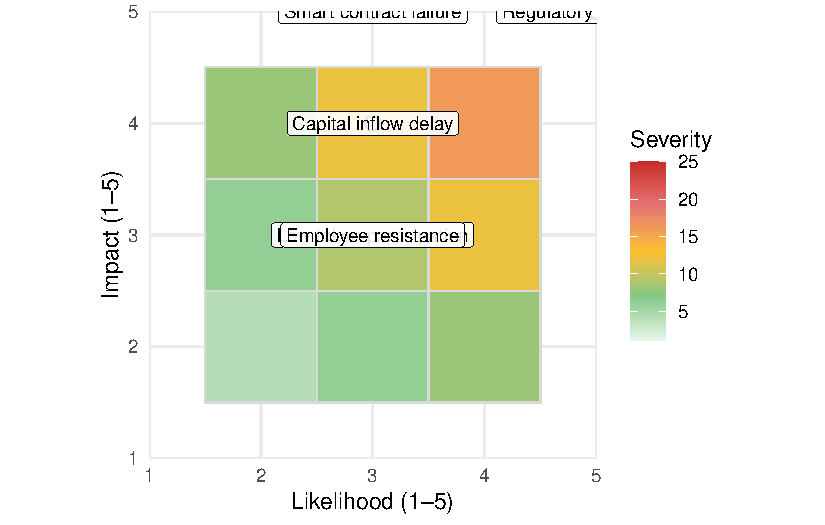
\includegraphics[keepaspectratio]{gp4_files/figure-pdf/risk-heatmap-appx-color-1.pdf}}

}

\caption{Risk heatmap for DAO-enabled governance at VIRIDIS.}

\end{figure}%

\section{Appendix B. Implementation Gantt Chart}\label{sec-gantt}

The Gantt chart visualises the timeline of the DAO implementation at
VIRIDIS across the four rollout phases. It highlights when major
deliverables are due and where dependencies align
(\citeproc{ref-european-commission-2019-financing-sustainable-growth}{Commission,
2019}).

\subsection{Timeline Overview}\label{timeline-overview}

\begin{itemize}
\tightlist
\item
  \textbf{Phase 1 (Q4 2025):} Preparation --- smart contract audit,
  dashboard beta, training.\\
\item
  \textbf{Phase 2 (Q1--Q2 2026):} Pilot advisory votes and reporting.\\
\item
  \textbf{Phase 3 (Q3 2026):} Controlled rollout with binding votes.\\
\item
  \textbf{Phase 4 (2027+):} Full DAO integration and oversight
  committee.
\end{itemize}

\subsection{Gantt Chart}\label{gantt-chart}

\begin{figure}[H]

{\centering \pandocbounded{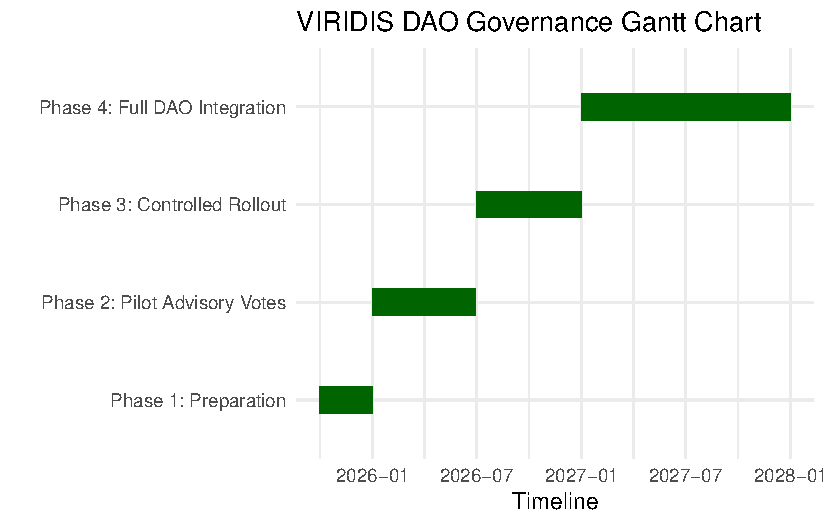
\includegraphics[keepaspectratio]{gp4_files/figure-pdf/gantt-chart-1.pdf}}

}

\caption{Implementation timeline for DAO governance at VIRIDIS.}

\end{figure}%

\section{Appendix C. Training Plan}\label{sec-training-plan}

The training plan equips employees, token holders, and partners with the
skills and confidence to engage effectively in DAO governance. It builds
literacy in both technical tools and participatory decision-making
(\citeproc{ref-atzori2018-trust-chain}{Atzori, 2018};
\citeproc{ref-tkachuk2023-efficient-design}{Tkachuk, 2023}).

\subsection{Training Objectives}\label{training-objectives}

\begin{itemize}
\tightlist
\item
  Build \textbf{capacity} among employees, managers, and token
  holders.\\
\item
  Ensure \textbf{literacy} in DAO processes, dashboard use, and
  compliance.\\
\item
  Foster a culture of \textbf{inclusivity and participatory governance}.
\end{itemize}

\subsection{Training Modules}\label{training-modules}

\begin{enumerate}
\def\labelenumi{\arabic{enumi}.}
\tightlist
\item
  \textbf{DAO Fundamentals} --- introduction to decentralised governance
  and token-based participation.\\
\item
  \textbf{Smart Contracts and Voting} --- functionality of VIA token,
  delegation rules, quorum thresholds.\\
\item
  \textbf{Dashboard Onboarding} --- navigation of proposals, casting
  votes, monitoring results.\\
\item
  \textbf{Regulatory and Compliance Basics} --- EU Taxonomy, SFDR, MiCA,
  and ESG-aligned reporting.\\
\item
  \textbf{Change Management} --- peer learning, DAO Champions, and
  bridging cultural resistance.
\end{enumerate}

\subsection{Schedule}\label{schedule}

\begin{itemize}
\tightlist
\item
  \textbf{Q4 2025}: Employee workshops and token holder orientation.\\
\item
  \textbf{Q1 2026}: Pilot training with simulations of voting flows and
  dashboard use.\\
\item
  \textbf{Q2 2026 onwards}: Quarterly refresher sessions and advanced
  modules.
\end{itemize}

\subsection{Participation Projection}\label{participation-projection}

\begin{figure}[H]

{\centering \pandocbounded{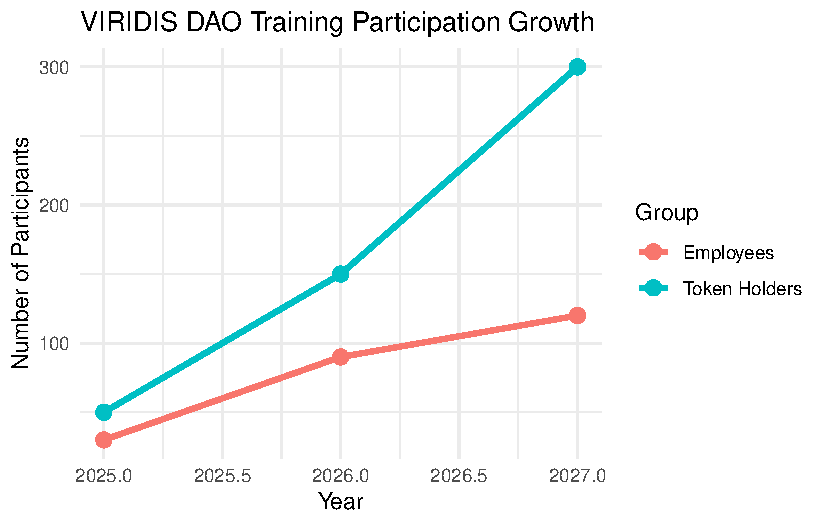
\includegraphics[keepaspectratio]{gp4_files/figure-pdf/training-participation-1.pdf}}

}

\caption{Projected growth of stakeholder training participation
(2025--2027).}

\end{figure}%

\section{Appendix D. Dashboard Mock-up}\label{sec-dashboard}

The governance dashboard will be the central interface for stakeholders
to access, participate, and monitor DAO-enabled governance at VIRIDIS.
It provides transparency by displaying proposals, votes, and financial
flows in real time
(\citeproc{ref-werner2020-governance-blockchain}{Werner et al., 2020}).

\subsection{Dashboard Features}\label{dashboard-features}

\begin{itemize}
\tightlist
\item
  \textbf{Proposal Overview}: List of active, pending, and closed
  proposals with status indicators.\\
\item
  \textbf{Voting Results}: Real-time vote tallies, quorum status, and
  outcome visualisations.\\
\item
  \textbf{Financial Flows}: On-chain records of approved budget
  allocations and project funding.\\
\item
  \textbf{Compliance Panel}: ESG alignment indicators linked to EU
  Taxonomy and SFDR disclosure requirements
  (\citeproc{ref-european-commission-2019-financing-sustainable-growth}{Commission,
  2019}).\\
\item
  \textbf{Participation Metrics}: Number of token holders voting,
  participation rates, and historical trends.
\end{itemize}

\subsection{Mock-up Example (Prototype
Data)}\label{mock-up-example-prototype-data}

\begin{figure}[H]

{\centering \pandocbounded{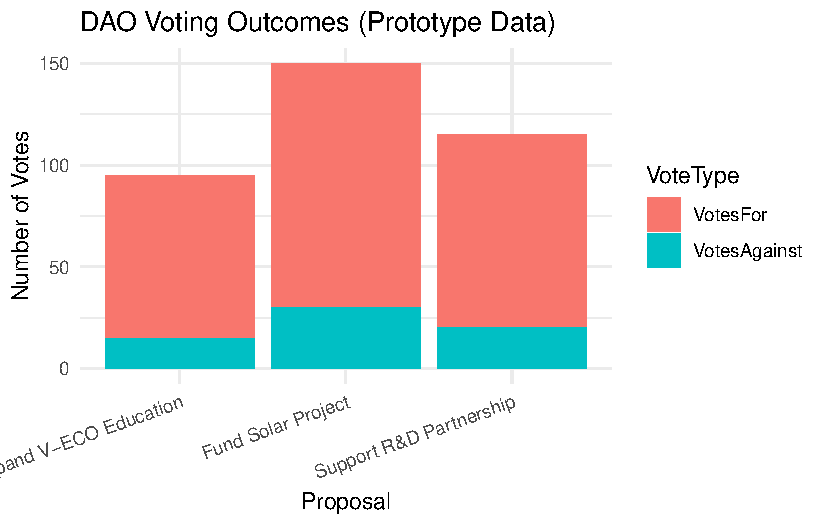
\includegraphics[keepaspectratio]{gp4_files/figure-pdf/dashboard-mock-1.pdf}}

}

\caption{Prototype visualisation of the VIRIDIS governance dashboard.}

\end{figure}%

This mock-up illustrates how voting results could be visualised on the
dashboard. Similar modules will track financial allocations, compliance
metrics, and participation levels, ensuring full transparency and
accountability.

\phantomsection\label{refs}
\begin{CSLReferences}{1}{0}
\bibitem[\citeproctext]{ref-aghion1997-decentralization}
Aghion, P., \& Tirole, J. (1997). Formal and real authority in
organizations. \emph{Journal of Political Economy}, \emph{105}(1),
1--29. \url{https://doi.org/10.1086/262063}

\bibitem[\citeproctext]{ref-atzori2018-trust-chain}
Atzori, M. (2018). Blockchain technology and decentralized governance:
The pitfalls of a trustless dream. \emph{Ledger}, \emph{3}, 38--54.
\url{https://doi.org/10.5195/ledger.2018.140}

\bibitem[\citeproctext]{ref-european-commission-2019-financing-sustainable-growth}
Commission, E. (2019). \emph{Factsheet: Financing sustainable growth}.
European Commission.

\bibitem[\citeproctext]{ref-kellers2022-mobilizing-capital}
Kellers, W. (2022). \emph{Mobilizing capital for sustainable impact:
Essays on sustainable finance}. University of Zurich.

\bibitem[\citeproctext]{ref-tkachuk2023-efficient-design}
Tkachuk, R.-V. (2023). \emph{Efficient design of decentralized privacy
and trust in distributed digital marketplaces} {[}PhD thesis{]}.
Blekinge Institute of Technology.

\bibitem[\citeproctext]{ref-viridis2025-financial-report}
VIRIDIS. (2025). \emph{Financial report 2025}.

\bibitem[\citeproctext]{ref-vonwachter2023-defi-phd}
Wachter, C. V. von. (2023). \emph{Decentralized finance: Building and
analyzing financial infrastructure on blockchain technology} {[}Ph.D.
thesis{]}. University of Copenhagen, Department of Computer Science.

\bibitem[\citeproctext]{ref-werner2020-governance-blockchain}
Werner, S. et al. (2020). Governance of blockchain systems: Trust,
transparency and participation. In \emph{Blockchain and the future of
governance} (pp. 45--62). Springer.

\end{CSLReferences}


\backmatter


\end{document}
